\documentclass{article}   
\usepackage[left=1.5cm,right=1.5cm,top=2.3cm,bottom=2.3cm]{geometry}		
\usepackage[utf8]{inputenc} 										
%\usepackage[french]{babel}
\usepackage{fancyhdr}								
\usepackage{hyperref}
\hypersetup{
    colorlinks=true,        % false: boxed links; true: colored links
    linkcolor=black,         % color of internal links (e.g., sections)
    citecolor=black,         % color of citation links
    filecolor=black,         % color of file links
    urlcolor=black           % color of external links
}								
\usepackage{booktabs,multirow,hhline}		
\usepackage{graphicx}				
\usepackage{bibentry}
%\usepackage{wrapfig,caption}
\usepackage{subcaption}
\usepackage[compact]{titlesec}
\titlespacing{\section}{0pt}{2ex}{1ex}
\titlespacing{\subsection}{0pt}{1ex}{0ex}
\titlespacing{\subsubsection}{0pt}{0.5ex}{0ex}
\usepackage{color}												
\usepackage[dvipsnames]{xcolor}								
\usepackage{amsmath,amssymb,amsthm,nicefrac}
\usepackage{mathrsfs}										
\usepackage{wasysym,marvosym}
\usepackage{mathtools}
\usepackage{verbatim}										
\usepackage{minted}										
\usepackage{lipsum}
\usepackage{tikz}
\usetikzlibrary{calc,patterns,angles,quotes}
\usepackage[american]{circuitikz}
\usepackage{siunitx}
\usepackage{physics}
\usepackage{float}
\usepackage{movie15}
\usepackage{multicol}
\usepackage{lineno}

\captionsetup[figure]{font=footnotesize, labelfont=bf}
\captionsetup[table]{font=footnotesize, labelfont=bf}

%\usepackage[backend=biber, style=numeric]{biblatex}
%\addbibresource{references.bib} %Imports bibliography file
\usepackage[super,sort]{natbib}

\renewcommand{\textfraction}{0.001} % Allows minimal text on a page
\renewcommand{\floatpagefraction}{0.999} % Requires float pages to be nearly full
\renewcommand{\topfraction}{0.999} % Allows the top of the page to be nearly all float
\renewcommand{\bottomfraction}{0.999} % Allows the bottom of the page to be nearly all float
\setcounter{totalnumber}{5}  % Maximum number of floats on a text page
\setcounter{topnumber}{3}    % Maximum number of floats at the top
\setcounter{bottomnumber}{2} % Maximum number of floats at the bottom

\parindent=0pt									
\parskip=6pt

\fancyheadoffset{0 cm}	

\linenumbers

%-------------------------------------------------------------------------------------------

\begin{document}

\begin{center}

    {\Large \textbf{Function aligns with geometry in locally connected neuronal networks}}\\
    
    \vspace{10 pt}
    \textbf{Antoine Légaré},$^{1,2}$ \textbf{Olivier Ribordy},$^{3,4}$, \textbf{Paul De Koninck}$^{1,2}$, \textbf{Antoine Allard},$^{1,3,4,*}$ \textbf{Patrick Desrosiers},$^{1,3,4,*}$ \\
    \vspace{5 pt}
    
    $^1$\textit{Centre de recherche CERVO, Québec (Qc), Canada.}\\
    $^2$\textit{Département de biochimie, de microbiologie et de bio-informatique, Université Laval, Québec (Qc), Canada}\\
    $^3$\textit{D\'epartement de physique, de g\'enie physique et d'optique, Universit\'e Laval, Qu\'ebec (Qc), Canada}\\% G1V 0A6}
    $^4$\textit{Centre interdisciplinaire en mod\'elisation math\'ematique de l'Universit\'e Laval, Qu\'ebec (Qc), Canada}\\
    $^*$\textit{Co-corresponding authors:} \href{mailto:patrick.desrosiers@phy.ulaval.ca}{patrick.desrosiers@phy.ulaval.ca}; \href{mailto:antoine.allard@nphy.ulaval.ca}{antoine.allard@phy.ulaval.ca}

\end{center}

\vspace{4 pt}

\hrulefill

\textbf{Abstract} - The geometry of the brain imposes fundamental constraints on its activity and function. However, the mechanisms linking its shape to neuronal dynamics remain elusive. Here, we investigate how geometric eigenmodes relate to functional connectivity gradients within three-dimensional structures using numerical simulations and calcium imaging experiments in larval zebrafish. We show that functional gradients arising from network activity closely match the geometric eigenmodes of the network’s spatial embedding when neurons are locally connected. By systematically varying network parameters such as the connectivity radius and the prevalence of long-range connections introduced via edge swaps, we reveal a robust geometry-function correspondence that progressively deteriorates as local connectivity is disrupted. Additionally, we demonstrate that spatial filtering can artificially impose geometric structure on functional gradients, even at modest levels. To support our computational results, we conduct volumetric calcium imaging experiments at cellular resolution in the optic tectum of zebrafish larvae. We uncover cellular functional gradients that closely align with geometric eigenmodes up to a certain eigenmode wavelength that reflects the spatial extent of neuronal arborizations measured in single-neuron reconstructions, as predicted by our simulations. Our findings highlight the importance of short-range anatomical connectivity in shaping the geometric structure of brain activity.

\hrulefill
\vspace{10 pt}

%\begin{multicols}{2}

\section*{Introduction}

Understanding what guides the flow of brain activity remains a central challenge in systems neuroscience. At any given moment, several factors influence brain dynamics, including external sensory inputs and ongoing internal demands\cite{flavell2022emergence}. However, the intrinsic structural connectivity of the brain imposes perhaps the most fundamental constraint on its activity\cite{suarez2020linking}. As in many natural systems, structure and function in the brain are deeply intertwined. Anatomical wiring diagrams can predict patterns of coordinated activity across neurons\cite{uzel2022set, randi2023neural, lappalainen2024connectome} or brain regions\cite{legare2025structural}, and the three-dimensional organization of neural populations across gyri, sulci, and subcortical nuclei reflects their functional specialization\cite{petersen2024principles}. A comprehensive understanding of how activity flows through the brain must therefore integrate both its network architecture and its spatial embedding---its geometry.

In human neuroimaging, network science is widely employed to model both anatomical connectivity and brain dynamics\cite{bassett2017network}. The most common network-based description of brain activity is functional connectivity (FC), typically defined as the correlation between activity time series from distinct brain regions. Although FC provides a compact statistical summary of interactions between neuronal populations over extended periods, it does not capture rapid, moment-to-moment fluctuations of the brain's activity\cite{zamani2020high}. Nonetheless, FC has proven useful: it reflects effective connectivity and is correlated with structural connectivity (SC), a relationship referred to as the structure-function coupling of brain networks\cite{fotiadis2024structure}. A recent and influential extension of FC analysis is the derivation of FC gradients that capture the dominant axes of variation in connectivity\cite{margulies2016situating, huntenburg2018large, bernhardt2022gradients}. These gradients have become powerful tools to examine the spatial organization of brain functions, not only in humans but also in animal models such as mice and zebrafish\cite{coletta2020network, legare2025structural}. While gradient analysis inherits the static nature of the FC matrix, the resulting spatial configurations offer insights into underlying dynamical processes. In particular, recent work has shown that a large portion of FC variance is driven by propagating waves of hemodynamic activity, which diffuse along canonical resting-state networks (RSNs) organized along the functional gradients\cite{yousefi2021propagating, raut2021global}. Thus, FC and its gradients appear to reflect the influence and directionality of spatially propagating activity, yet the mechanisms shaping these statistical patterns remain incompletely understood.

Across a wide range of recording modalities and animal models, waves of neuronal activity have been consistently observed in both cortical and subcortical structures\cite{raut2021global, ye2023brain, matsui2016transient, xu2023interacting}. While their precise origins and computational roles remain debated, these waves likely emerge from fundamental architectural features such as conduction delays and the prevalence of short-range connectivity\cite{muller2018cortical}. A hallmark of brain networks is wiring length minimization, which favors local connections between neurons or brain regions\cite{bullmore2012economy}. Although long-range projections are essential to coordinate global dynamics\cite{o2013causal, betzel2018specificity, vohryzek2025human}, their relative sparsity suggests that much of brain activity arises from local interactions. Neural Field Theory (NFT) formalizes this idea by modeling brain activity as the propagation of electrical waves across a continuous neural sheet\cite{robinson1997propagation, robinson2016eigenmodes, gabay2018dynamics}, typically governed by an exponential decay rule (EDR) of connectivity\cite{ercsey2013predictive}. A recent study by Pang and colleagues\cite{pang2023geometric} used noninvasive MRI to test a key prediction of NFT: that cortical geometry itself imposes constraints on activity propagation beyond those imposed by white matter connectivity. Supporting this hypothesis, they showed that geometric eigenmodes of the Laplace-Beltrami operator (LBO) on the cortical surface offer a parsimonious basis to reconstruct brain activation patterns\cite{pang2023geometric}. Remarkably, a one-to-one correspondence was observed between geometric eigenmodes and FC gradients in subcortical structures, where their shape alone predicted the dominant axes of variation in connectivity\cite{pang2023geometric}. These findings underline the strong influence of geometry on brain function, yet the generative mechanisms linking geometry, connectivity, and activity remain elusive. Moreover, the limited spatial resolution of fMRI, together with common preprocessing steps such as spatial filtering, can introduce biases in gradient analyses\cite{watson2023connectopic}, underscoring the need for validation in alternative animal models where such confounds are absent.

In this study, we combine numerical simulations and optical imaging at cellular resolution to investigate the link between FC gradients and geometric eigenmodes in brain networks. Using simulations of neuronal networks embedded in various 3D shapes, we show that the correspondence between FC gradients and geometric eigenmodes emerges naturally from short-range connectivity and local correlations, independent of specific spatiotemporal dynamics. We further demonstrate that this correspondence deteriorates as local connectivity is disrupted, revealing a wavelength-dependent decay of the eigenmode-gradient correlations that serves as a sensitive readout of the spatial extent of underlying anatomical connections. To validate our numerical findings and extend previous neuroimaging results\cite{pang2023geometric}, we perform two-photon calcium imaging in the larval zebrafish optic tectum, a brain structure with local recurrent connectivity. We observe functional gradients that coincide with the geometric eigenmodes of the tectum and, consistent with our simulations, the cutoff point of this mapping predicts the median arbor size of morphologically reconstructed tectal neurons with micron-level precision\cite{kunst2019cellular}. Altogether, our results identify a simple generative mechanism for the emergence of geometric connectivity gradients and statistical patterns in the brain, and underscore the prevailing influence of geometry on both anatomical wiring and functional organization.

\section*{Results}

Throughout this study, we compare geometric eigenmodes and FC gradients (henceforth also referred to as eigenmodes and gradients, respectively) in neuronal populations embedded within three-dimensional volumes of various shapes. Geometric eigenmodes are the eigenvectors of the Laplace–Beltrami operator (LBO, Methods), and capture spatial patterns---analogous to vibrational modes---that arise from the shape of the embedding. FC gradients are computed from pairwise activity correlations using diffusion maps\cite{Coifman2006}, and represent principal axes of connectivity variation in the network (Methods). When applied to brain connectivity data, FC gradients spatially map onto different brain functions, providing a data-driven measure of functional organization\cite{margulies2016situating}. Importantly, eigenmodes and gradients are two independently derived measures of the same system. Their correspondence thus reflects how functional specialization aligns with the geometry of the volume in which the network is embedded.

\subsection*{Gradients and eigenmodes in locally connected networks}

\begin{figure*}[t]
    \centering
    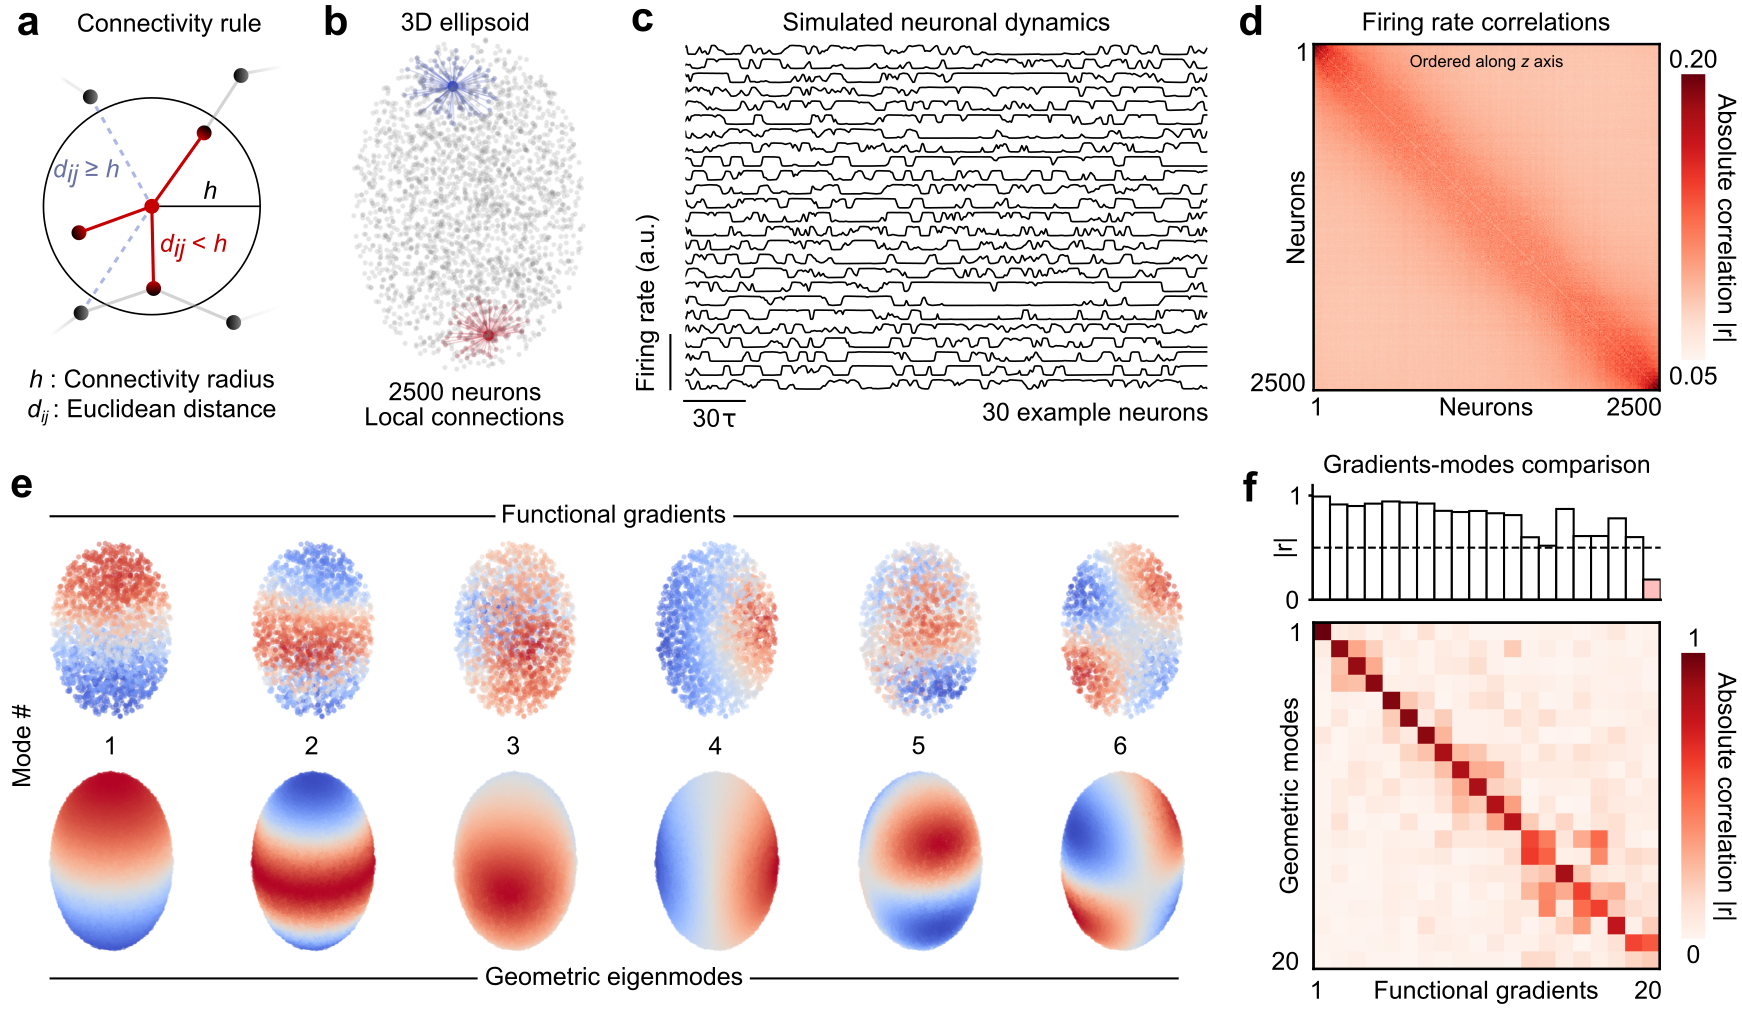
\includegraphics[width=1.0\linewidth]{figures/figure1.pdf}
    \caption{Geometric gradients emerge in firing rate networks with local connectivity. (\textbf{a}) Illustration of the connectivity rule wherein two nodes are connected if and only if separated by Euclidean distance less than $h$. (\textbf{b}) Centroids of 2500 neurons in a 3D ellipsoid; example local connectivity profiles with $h=0.1$ are highlighted in red and blue. (\textbf{c}) Example of one simulation of the firing rate dynamics with 50 neurons. (\textbf{d}) Average correlation matrix from 250 simulations (FC); neurons are ordered along the major axis (vertical) of the ellipsoid. (\textbf{e}) Top row, six functional gradients obtained using diffusion eigenmap, ordered based on their correlation with geometric modes; bottom row, first six geometric eigenmodes of the ellipsoid, with the first constant eigenmode excluded. (\textbf{f}) Bottom, absolute correlation matrix of the first 20 eigenmode-gradient pairs, after functional gradients have been optimally mapped to geometric eigenmodes; top, absolute correlations of the optimally mapped eigenmodes (diagonal of the matrix below); a dashed line indicates an intermediate $|r|=0.5$ correlation.}
    \label{fig1}
    \hrulefill
\end{figure*}

To explore the relationship between gradients and eigenmodes, we first simulated neuronal population dynamics in various three-dimensional geometries, understood here as Riemannian manifolds embedded in Euclidean space. Neurons were assigned random coordinates within each geometry, then connected if separated by a distance shorter than a threshold distance, $h$, that we call the network's connectivity radius (Fig. \ref{fig1}\textbf{a}). As a first case study, we generated a simple 3D ellipsoid with $N=2500$ locally connected neurons with $h=0.1$, corresponding to 10\% of the system’s characteristic length (Fig. \ref{fig1}\textbf{b}). We randomly assigned a weight to each connection and then simulated simple chaotic firing rate dynamics resulting from nonlinear excitatory and inhibitory interactions between connected neurons (Fig. \ref{fig1}\textbf{c}, Methods). We then computed an average correlation matrix $C$ from the firing rates of neurons by averaging the absolute value of the pairwise correlations from a large number of simulations, throughout which node coordinates and connections were preserved, but weights and initial conditions were drawn randomly each time. Correlations were generally higher between neurons situated at roughly the same position along the major axis (vertical) of the ellipsoid (Fig. \ref{fig1}\textbf{d}), suggesting the emergence of spatial patterns in the activity within the geometry. We computed functional gradients from the averaged $C$ matrix using the diffusion maps method\cite{Coifman2006}, revealing smooth spatial functions once projected onto network nodes (Fig. \ref{fig1}\textbf{e}, top row, Methods). Independently, we numerically evaluated the geometric eigenmodes of the ellipsoid (Fig. \ref{fig1}\textbf{e}, bottom row, Methods), and correlated them with functional gradients after finding an optimal linear mapping between both mode ensembles (Fig. \ref{fig1}\textbf{f}, Methods). We observed a strong correspondence between eigenmodes and gradients, with correlations exceeding $|r|=0.5$ for the first 19 mode pairs. In contrast, this eigenmode-gradient correspondence vanished in networks where local connections were shuffled, preserving the network density and connection weights but removing the distance-dependence of connectivity (data not shown). This simple first case study demonstrates that \emph{geometric gradients}---FC gradients that correlate strongly with geometric eigenmodes---emerge readily from the activity of locally connected networks. This result is not a consequence of the simplicity of the ellipsoid geometry, as geometric gradients could also be observed in more complex geometries (Supp. Fig. \ref{supp_geometries}). 

\subsection*{Geometric gradients emerge irrespective of network dynamics}

To further generalize the previous observations, we conducted simulations of network activity within the same ellipsoid, but using different dynamical models (Supp. Fig. \ref{supp_dynamics}, Methods): chaotic firing rate neurons\cite{sompolinsky1988chaos, rajan2010stimulus}, with and without Dale's law enforced on the connectivity matrix (models 1 \& 2), Kuramoto-Sakaguchi (KS) oscillators\cite{sakaguchi1986soluble} (model 3), binary stochastic neurons (model 4), and spiking leaky integrate-and-fire (LIF) neurons with simple calcium dynamics\cite{izhikevich2007dynamical} (model 5). Despite very different activity profiles (Supp. Fig. \ref{supp_dynamics}\textbf{a}, Supp. Video. 1), each model yielded local and spatially decaying correlations (Supp. Fig. \ref{supp_dynamics}\textbf{b}-\textbf{c}), and the functional gradients calculated from their averaged correlation matrices were strongly correlated with the ellipsoid's geometric eigenmodes (Supp. Fig. \ref{supp_dynamics}\textbf{d}, averages of 10 random coordinate sets per volume). Gradients derived from the two firing rate models correlated significantly more with geometric eigenmodes than the other three models (Supp. Fig. \ref{supp_dynamics}\textbf{e}, $P<10^{-4}$, one-way ANOVA), with KS oscillators performing the worse, possibly due to the presence of more spurious correlations between oscillators. Indeed, across all five dynamical models, we observed a strong positive relationship between the strength of the correlation-distance relationship, and the quality of the eigenmode-gradient correspondence, quantified by averaging the absolute correlation $|r|$ across the first 50 mode pairs (Supp Fig. \ref{supp_dynamics}\textbf{f}, Pearson $r=0.798$). This suggests that geometric gradients are degraded when activity correlations are not as tightly linked to Euclidean distance. Importantly, none of the above models explicitly implement wave dynamics---a presumed mechanism for the emergence of geometry in functional measurements\cite{pang2023geometric}---although waves can sporadically be perceived within their chaotic dynamics (Supp. Video. 1). These results suggest that wave-like dynamics are not a prerequisite for the emergence of geometric gradients. Rather, the predominant locality of connections and correlations between neurons, regardless of their dynamical regime, is sufficient to drive this phenomenon.

\subsection*{Geometric gradients vanish rapidly as the connectivity radius increases}

Known theoretical results support our previous observations. For random geometric networks whose nodes are sampled from a smooth underlying manifold, it has been demonstrated that the eigenvectors of the graph laplacian converge to the eigenmodes of the LBO as $N\to \infty$ and $h\to 0$\cite{GarcaTrillos2019}. Diffusion maps, used here to compute gradients, are parameterized by a value $\alpha \in [0, 1]$, which dictates how strongly sample density is taken into account (Methods). At $\alpha=0$, the diffusion maps used to derive gradients directly correspond to the random-walk normalized graph laplacian. At $\alpha = 1$, the diffusion maps approximate the LBO itself, with convergence obeying the same conditions of dense locality as for the graph laplacian\cite{Coifman2006}. While there are a few methodological differences between these theoretical results and our network simulations, we observe an alignment between gradients and eigenmodes in locally connected networks across all parameterizations of the diffusion maps (Methods, Supp. Fig. \ref{supp_methods}\textbf{a}). Moreover, other gradient derivation methods commonly used in the neuroimaging literature similarly yield geometric gradients (Supp. Fig. \ref{supp_methods}\textbf{b}-\textbf{c}), thereby suggesting that the theoretical convergence results extend beyond the asymptotic regime to different methodologies. Theory also predicts that the correspondence between gradients and eigenmodes should break apart rapidly as the connectivity radius increases, with the quality of the correspondence proportional to $\sim 1/h^3$ for 3-dimensional structures.

To characterize the sensitivity of the eigenmode-gradient correlation, we next evaluated the effect of network size $N$ and connectivity radius $h$ on the geometry-function correlation, quantified by averaging absolute correlations through 50 pairs of modes. For a fixed $h=0.1$, we found that the average eigenmode-gradient correlation increased with network size $N$, with larger networks providing a denser sampling of the geometry (Supp. Fig. \ref{supp_network_size}). For a fixed size of $N=2500$, increasing the connectivity radius $h$ rapidly decreased the correlation (Fig. \ref{fig2}\textbf{b}). At small $h$ values, we observed a reduced eigenmode-gradient correlation, corresponding to a regime where networks are too disconnected to properly sustain network dynamics. By further increasing $h$, the correlation increased rapidly, peaking at roughly $h=0.08$ before decreasing again. We estimated the rate of divergence between eigenmodes and gradients by subsampling individual simulation results from the decaying portion of the curve and then fitting $1/h^m$ curves (Fig. \ref{fig2}\textbf{c}). This procedure generated an average power law exponent of $m=2.69\pm0.11$, close to the theoretical value of $m=3$ and underlining a rapid decrease of eigenmode-gradient correlation as the connectivity radius increases (mean $\pm$ standard deviation, Fig. \ref{fig2}\textbf{d}, 10000 bootstrap estimates, Methods). Our numerical observations thus agree qualitatively and quantitatively with previous analytical results\cite{GarcaTrillos2019}. For large $N$ and small $h$, eigenmodes and gradients are similar, but when these conditions are broken, the average correlation decreases rapidly with an exponent nearing $m\approx3$.

\subsection*{Geometric gradients are robust to long-range connections}

Brain networks are characterized by the presence of long-range connections that dramatically improve routing efficiency while allowing the integration of functionally diverse inputs across distant brain regions\cite{betzel2018specificity}. The random geometric network model used so far lacks this important topological feature, focusing solely on the effect of local connections. Moreover, increasing the connectivity radius $h$ has the confounding effect of also increasing the network's density (Fig. \ref{fig2}\textbf{a}). Therefore, we next evaluated the effect of introducing double edge swaps in networks that were initially locally connected, a procedure that gradually and randomly introduced long range connections, without changing the network's density (Fig. \ref{fig2}\textbf{e}). To ensure a monotonous increase in the average connection distance $d$ between nodes (Fig. \ref{fig2}\textbf{f}), we prevented swaps that would result in links shorter than the initial connectivity radius $h$, which was set to $h=0.1$. Similar to the effect of gradually increasing $h$, increasing the fraction of swapped edges $\rho_{\text{swaps}}$ led to a decrease in the average eigenmode-gradient correlation $|r|$ (Fig. \ref{fig2}\textbf{g}), further emphasizing the importance of local connections. Interestingly, we observed a slower, sublinear decay of $|r|$ (Fig. \ref{fig2}\textbf{g}), with gradients remaining highly correlated with eigenmodes even with $10-20\%$ of the edges swapped. To compare this with the effect of increasing $h$, we plotted the average eigenmode-gradient correlation $|r|$ as a function of the average connection distance $d$ within networks obtained through either connectivity radius expansion or double edge swaps (Fig. \ref{fig2}\textbf{h}). At similar average connection lengths, edge swapping retained a much higher eigenmode-gradient correlation, even though some of the swapped edges could in theory span the entire length of the system. 

These results demonstrate that, while a backbone of local connectivity is necessary, the eigenmode-gradient correspondence is robust to the presence of a small fraction of random, potentially long range connections. As the average distance between connected neurons increases, however, the correspondence eventually vanishes, regardless of the underlying network topology. Interestingly, these results imply that real neuronal networks, despite the presence of many long-range connections, could exhibit geometric gradients, since most of their connections are local in space\cite{ercsey2013predictive}.

\begin{figure*}[t]
    \centering
    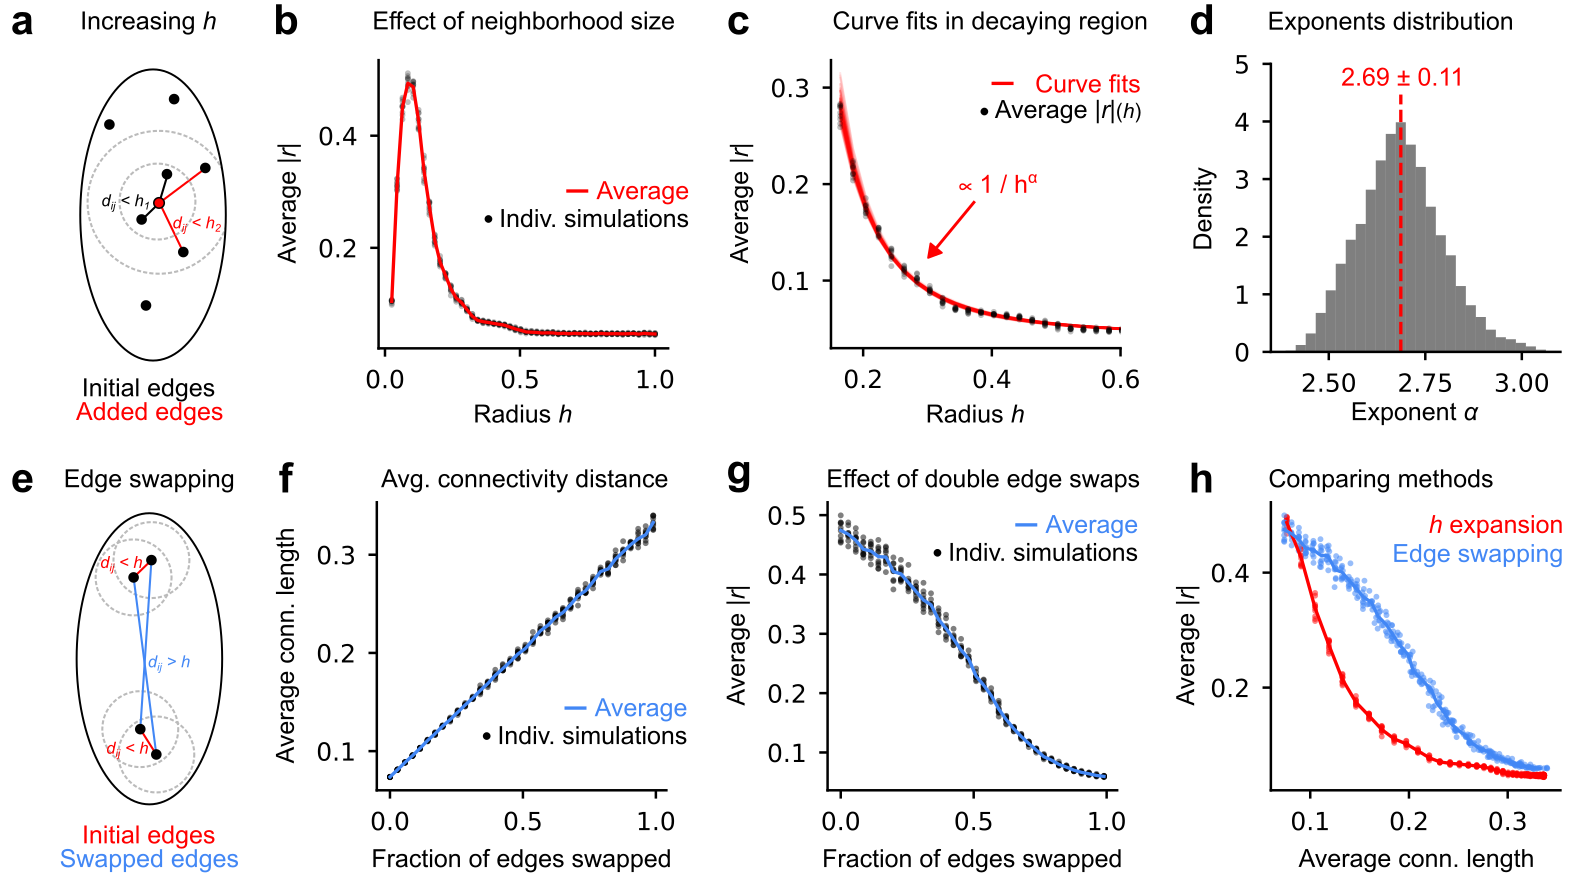
\includegraphics[width=1.0\linewidth]{figures/figure2.pdf}
    \caption{Eigenmode-gradient correlation decreases as connectivity neighborhood increases. (\textbf{a}) Increasing the connectivity radius $h$ adds longer edges to the network. (\textbf{b}) Average absolute Pearson correlation $|r|$ as a function of connectivity radius $h$; 10 simulations per $h$ value. (\textbf{c}) Power-law curve fits in the decaying region of the previous panel; the exponents are estimated from randomly selected individual simulations at each $h$ value. (\textbf{d}) Distribution of fitted exponents $m$ obtained through bootstrapping and curve fitting individual simulations; a dashed red line indicates the distribution average. (\textbf{e}) Schematization of the double edge swapping procedure; two randomly selected edges (in red) are swapped such that their new lengths (in blue) exceed the initial connectivity radius $h$. (\textbf{f}) Average connection length as a function of the fraction of swapped edges; 10 simulations performed for each fraction of edges swapped. \textbf{g}) Average geometry-function correlation $|r|$ as a function of the fraction of swapped edges; 10 simulations per fraction of edges swapped. (\textbf{h}) Comparison of the decrease in $|r|$ as a function of average connection length, achieved either by increasing $h$ (in red) or by swapping edges (in blue).}
    \label{fig2}
    \hrulefill
\end{figure*}

\subsection*{Small wavelength eigenmodes progressively disappear as the connectivity radius increases}

We investigated the effects of increasing $h$ or swapping edges on the correlation of \emph{single} eigenmodes with their corresponding gradients. By visual inspection, a gradual increase in the connectivity radius $h$ led to the disappearance of small wavelength modes (Fig. \ref{fig3}\textbf{a}, average of 10 simulations per matrix, $N=1500$ neurons). Conversely, the first, higher-wavelength modes were resilient to this parameter change. At sufficiently large values of $h$, only the first geometric gradient persisted, but further increases in $h$ completely eliminated the correspondence (Fig. \ref{fig3}\textbf{a}, right). To more appropriately visualize the effect of $h$ on individual eigenmodes, we plotted the diagonals of the correlation matrix at varying connectivity radii (Fig. \ref{fig3}\textbf{b}). The presence of abrupt cutoff points suggests that each individual geometric gradient exists only under a certain connectivity radius threshold. We estimated the positions of cutoff points for each of the first 50 mode pairs by identifying the value of $h$ corresponding to the maximal negative slope of $|r_i|(h)$ (red arrows show these cut off points for the first modes in Fig. \ref{fig2}\textbf{b}, Methods). We then compared these cutoff points to the approximate wavelengths $\lambda_i$ of each eigenmode (estimated from geometric eigenmode variograms, Supp. Fig. \ref{supp_variograms}, Methods), and observed a strong linear relationship (Fig. \ref{fig3}\textbf{c}, $R^2=0.964$). Thus, the spatial extent of neuronal connections sets a fundamental resolution limit beyond which geometric gradients cannot be observed.

We conducted a similar analysis for simulated networks which underwent double edge swaps that introduced long-range connections. In this case, increasing the fraction of swapped edges $\rho_{\text{swaps}}$ led to more uniform decrease of individual eigenmode-gradient correlations, with complete matrix diagonals still visible with 20\% of edges swapped (Fig. \ref{fig3}\textbf{d}). We plotted the correlation matrix diagonals against varying $\rho_{\text{swaps}}$ (Fig. \ref{fig3}\textbf{e}), thereby confirming the absence of clear cutoff points beyond which individual geometric gradients abruptly disappear. Rather, each eigenmode-gradient pair undergoes a linear decrease of its correlation with $\rho_{\text{swaps}}$. As a consequence, there was no clear relationship observed between maximal slope cutoff points and eigenmode wavelengths (Fig. \ref{fig3}\textbf{f}, $R^2=0.391$). These results suggest that edge swapping leads to a gradual distortion of all geometric gradients at once, rather than the abrupt disappearance of individual eigenmodes (see Supp. Fig. \ref{supp_lineprofiles}\textbf{a}-\textbf{c} for a side-by-side comparison).

Altogether, these results show that the minimal wavelength of geometric gradients approximately follows a linear relationship with the network's connectivity radius. As connections extend further in space, geometric gradients with shorter wavelengths first disappear, while long-wavelength gradients remain largely preserved. This result implies that in real neuronal networks, where connections extend over non-negligible distances, there should be an observable cutoff point beyond which eigenmodes and gradients no longer correspond.

\subsection*{Spatial filtering artificially induces geometric gradients}

Our numerical experiments so far demonstrate how the correspondence between eigenmodes and gradients is driven by short-range neuronal connections. A key implication is that any processing step that amplifies local connectivity measures can bias this relationship. Spatial filtering, a ubiquitous step in MRI preprocessing pipelines, blends signals from neighboring voxels, thereby enhancing local correlations. In a recent study\cite{watson2023connectopic}, spatial filtering was shown to artificially induce smooth spatial gradients in functional MRI data, which could be misidentified as meaningful connectopies\cite{haak2018connectopic}. This bias was accentuated when considering functional gradients at a smaller spatial scale within individual brain regions. 

\begin{figure}[t]
    \centering
    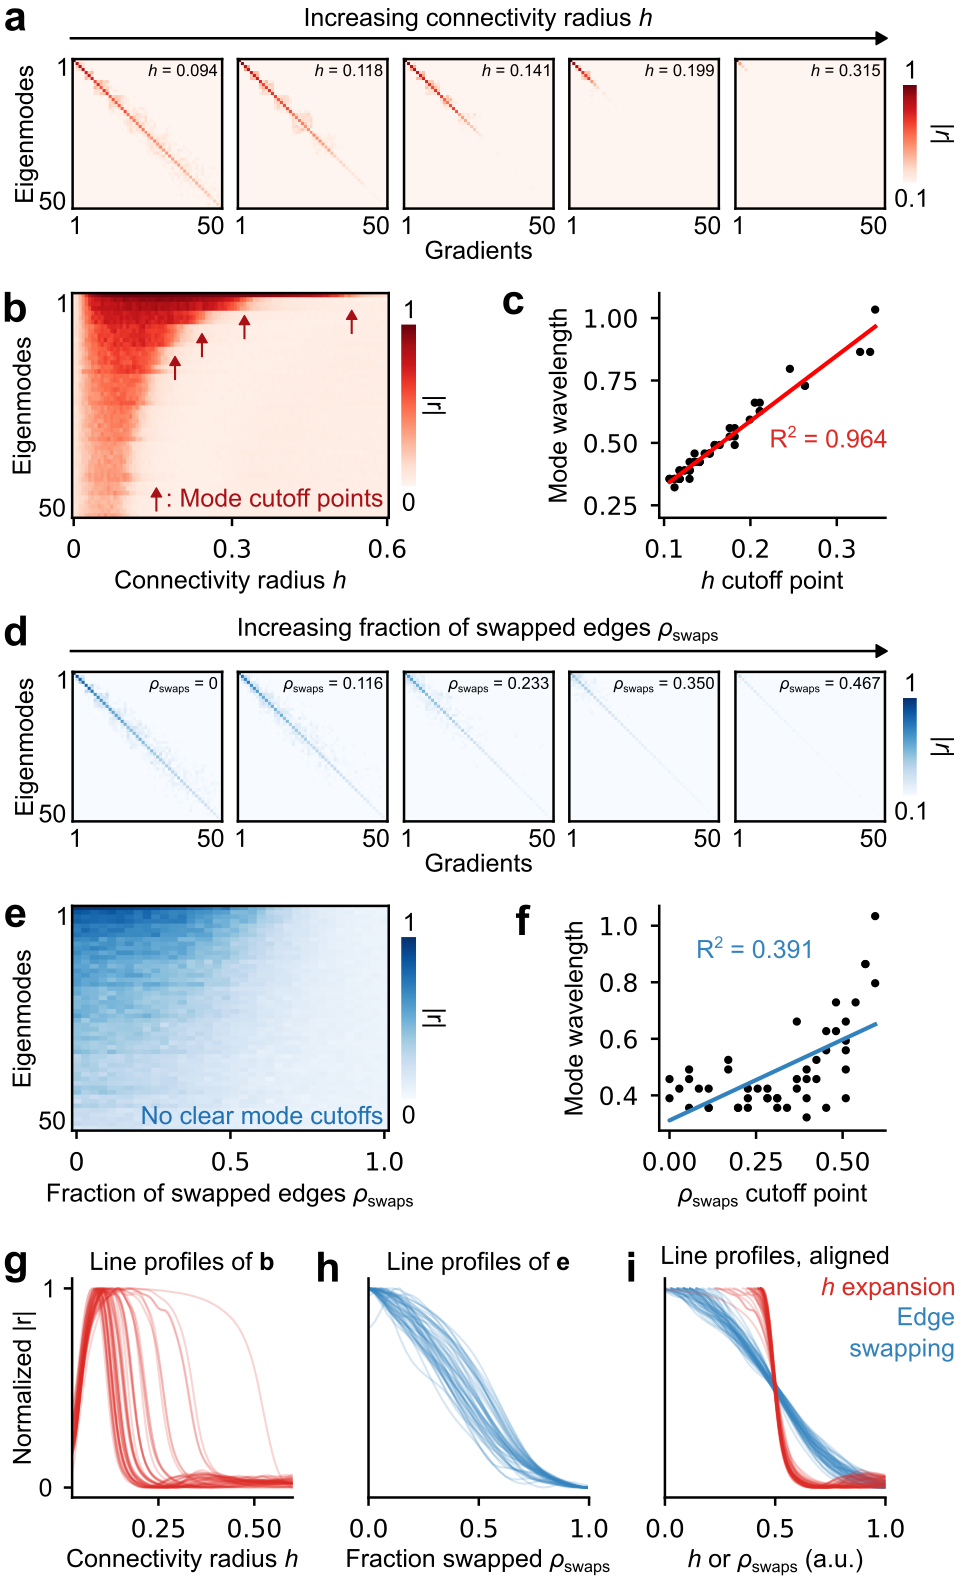
\includegraphics[width=1.0\linewidth]{figures/figure3.pdf}
    \caption{Degradation of higher spatial frequency geometric eigenmodes as connectivity radius increases. (\textbf{a}) Five example eigenmode-gradient correlation matrices for increasing connectivity radii $h$; each matrix is averaged across 10 different coordinate ensembles within the ellipsoid ($N=1500$ neurons, 100 averaged simulations per coordinate set). (\textbf{b}) Eigenmode-gradient correlation matrix diagonals (columns) for various $h$; arrows denote locations where eigenmode-gradient correlations abruptly drop. (\textbf{c}) Linear relationship between estimated eigenmode wavelengths and the $h$ cutoff points. (\textbf{d}) Five example eigenmode-gradient correlation matrices for increasing fractions of swapped edges $\rho_{\text{swaps}}$; similar averaging parameters as panel \textbf{a}. (\textbf{e}) Eigenmode-gradient correlation matrix diagonals (columns) at varying fractions of swapped edges; notice the absence of abrupt correlation decays. (\textbf{f}) Relationship between estimated eigenmode wavelengths and the $\rho_{\text{swaps}}$ cutoff points.}
    \label{fig3}
    \hrulefill
\end{figure}

To evaluate the influence of spatial filtering on geometric gradients, we substituted the simulated activity of neurons within the ellipsoid with uncorrelated Gaussian noise signals (Fig. \ref{fig4}\textbf{a}). We spatially filtered the noisy signals using a Gaussian kernel (Fig. \ref{fig4}\textbf{b}), combining uncorrelated signals from nearby neurons according to a single parameter $\sigma$ dictating the width of the gaussian kernel (Methods). By design, spatial filtering with a small kernel size of $\sigma=0.05$ introduced high artificial correlations between nearby neurons (Fig. \ref{fig4}\textbf{c}). We computed functional gradients from both unfiltered and filtered correlation matrices, revealing strikingly smooth gradients in the filtered case (Fig. \ref{fig4}\textbf{d}). These filtering-induced gradients were strongly correlated with the geometric eigenmodes of the ellipsoid (average $|r|=0.793$ across 20 modes; $|r|=0.604$ across 50 modes; Fig. \ref{fig4}\textbf{e}). This simple analysis demonstrates that geometric gradients can be artificially induced by spatial filtering, even in the complete absence of correlation between the raw signals.

\begin{figure*}[t]
    \centering
    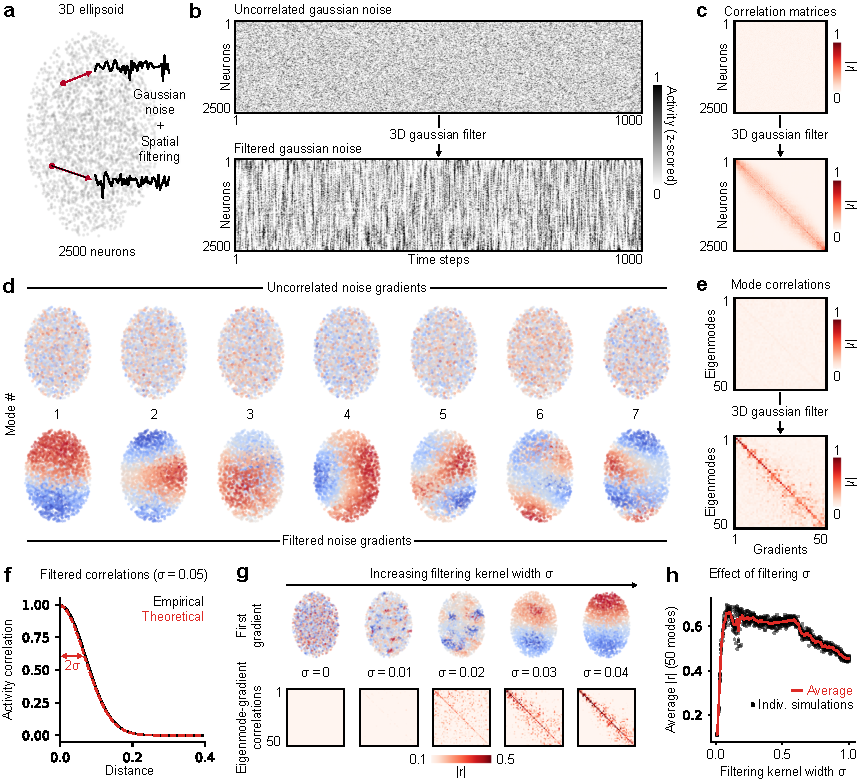
\includegraphics[width=1.0\linewidth]{figures/figure4.pdf}
    \caption{Spatial filtering of gaussian noise yields geometric gradients. (\textbf{a}) Schematization of the "simulations" for the noise filtering analysis; random gaussian noise signals are assigned 3D coordinates within an ellipsoid, then spatially filtered. (\textbf{b}) Top, matrix of random gaussian signals; bottom, same matrix after spatial filtering with $\sigma=0.05$; neurons are ordered along the $z$ axis. (\textbf{c}) Correlation matrix between noisy signals, before (top) and after (bottom) spatial filtering. (\textbf{d}) First 6 functional gradients before (top) and after (bottom) spatial filtering. (\textbf{e}) Correlation matrices between eigenmodes and gradients before (top) and after (bottom) spatial filtering. (\textbf{f}) Distributions for theoretical (dashed red line) and empirical (black line) correlations between spatially filtered signals based on the distance between nodes. (\textbf{g}) First gradient (top) and eigenmode correlation matrices (bottom) for increasing filtering kernel sizes $\sigma$. (\textbf{h}) Average eigenmode-gradient correlation $|r|$ (first 50 modes/gradients) for varying kernel sizes $\sigma$; black dots correspond to individual simulations (10 per $\sigma$ value, $N=1500$ neurons), while the red curve is the average. Notice a notch at roughly $\sigma=0.2$, which is likely an artifact of numerical discretization.}
    \label{fig4}
    \hrulefill
\end{figure*}

 We next investigated the sensitivity of this effect to the width of the filtering kernel $\sigma$. First, we derived an analytical approximation for the filtering-induced correlations $\Tilde{c}$ between two uncorrelated time series, encapsulated in the simple relationship $\Tilde{c}\approx e^{-\nicefrac{d^2}{4\sigma^2}}$ where $d$ is the distance that separates both nodes (see Supplementary Mathematical Note). This relationship is exact in the limit of an infinite and homogeneous system. Crucially, the width of the filtering-induced correlation Gaussian is $\sqrt{2}\sigma$, larger than the initial filtering kernel width. We validated this relationship numerically for small $\sigma=0.05$ relative to the full size of the system, where border effects are more negligible (Fig. \ref{fig4}\textbf{f}, $N=3000$ neurons embedded in 3D ellipsoid). This result suggests that spatial filtering induces correlations that deceptively extend beyond the spatial footprint of the kernel. To further explore the implications on functional gradients, we evaluated the effect of $\sigma$ on the average eigenmode-gradient correlation, observing the rapid emergence of smooth geometric gradients from very small filtering kernels (Fig. \ref{fig4}\textbf{g}, top). These smooth gradients were strongly correlated with geometric eigenmodes across all 50 mode pairs considered (Fig. \ref{fig4}\textbf{g}, bottom). In Fig. \ref{fig4}\textbf{h}, we plot the average eigenmode-gradient correlation $|r|$ for $\sigma$ ranging from $0$ to $1$, highlighting the very abrupt emergence of geometry with increasing $\sigma$ from purely noisy signals. Interestingly, eigenmode-gradient correlations remained high and decreased slightly for higher $\sigma$ values that approached the characteristic length of the ellipsoid. This behavior contrasts with the effect of increasing the connectivity radius $h$, as the eigenmode-gradient correspondence here persisted at large kernel sizes.
 
 These results underscore the high sensitivity of geometric gradients to spatial filtering, with artificial geometric features emerging from very small filtering kernels, consistent with previous reports on the confounding effects of spatial filtering in MRI studies \cite{watson2023connectopic}. This raises concerns about potential biases when interpreting geometric features in imaging modalities that rely on spatial filtering, particularly within small or spatially compact brain structures.

\subsection*{Differential effects of combined local connectivity and spatial filtering in simulations}

The previous results considered an unrealistic case where there are no correlations in the raw signals. To investigate the potentially nonlinear effects of filtering applied to a system exhibiting non-trivial correlations, we returned to simulated firing rate dynamics in locally connected networks, and then applied increasing amounts of spatial filtering to neuronal time series (Fig. \ref{fig5}\textbf{a}) before computing pairwise correlations (Fig. \ref{fig5}\textbf{b}). We evaluated the average eigenmode-gradient correlation for different combinations of $h$ and $\sigma$ ranging from $h=0.1$ to $h=0.6$, and $\sigma=0$ to $\sigma=0.1$ (Fig. \ref{fig5}\textbf{c}, 10 ellipsoids per parameterization). The different line profiles of the $(h, \sigma)$ grid in Fig. \ref{fig5}\textbf{c} can be visualized in Fig. \ref{fig5}\textbf{d}, where a differential effect of filtering is observed, depending on the initial value of $h$. In the case where connections are non-local ($h\approx0.6$), the unfiltered eigenmode-gradient correlation is marginal ($|r|<0.1$), but increases steadily as filtering is applied (Fig. \ref{fig5}\textbf{c}, bottom rows; Fig. \ref{fig5}\textbf{c}, bottom curves). When network connections are moderately local ($h\approx0.3$), a limited eigenmode-gradient correlation is initially present. In this case, increasing the filtering kernel width has no effect until a certain kernel size is reached (Fig. \ref{fig5}\textbf{c}, middle rows; Fig. \ref{fig5}\textbf{c}, middle curves). A perhaps counterintuitive effect is observed for the most locally connected systems ($h\approx0.1$), as spatial filtering decreases the initially high eigenmode-gradient correlation (Fig. \ref{fig5}\textbf{c}, top rows; Fig. \ref{fig5}\textbf{c}, top curves). Beyond a certain filtering kernel size ($\sigma>0.05$), all systems exhibit monotonically increasing correlations between eigenmodes and gradients, with filtering-induced correlations seemingly taking over correlations in the raw, unfiltered signals, if any. Altogether, these results highlight the differential and nonlinear effects of spatial filtering on correlated systems. While geometric gradients are amplified by excessive spatial filtering, the magnitude of this effect may be dependent on the initial locality of connections and correlations within the 3D geometry.

\begin{figure*}[t]
    \centering
    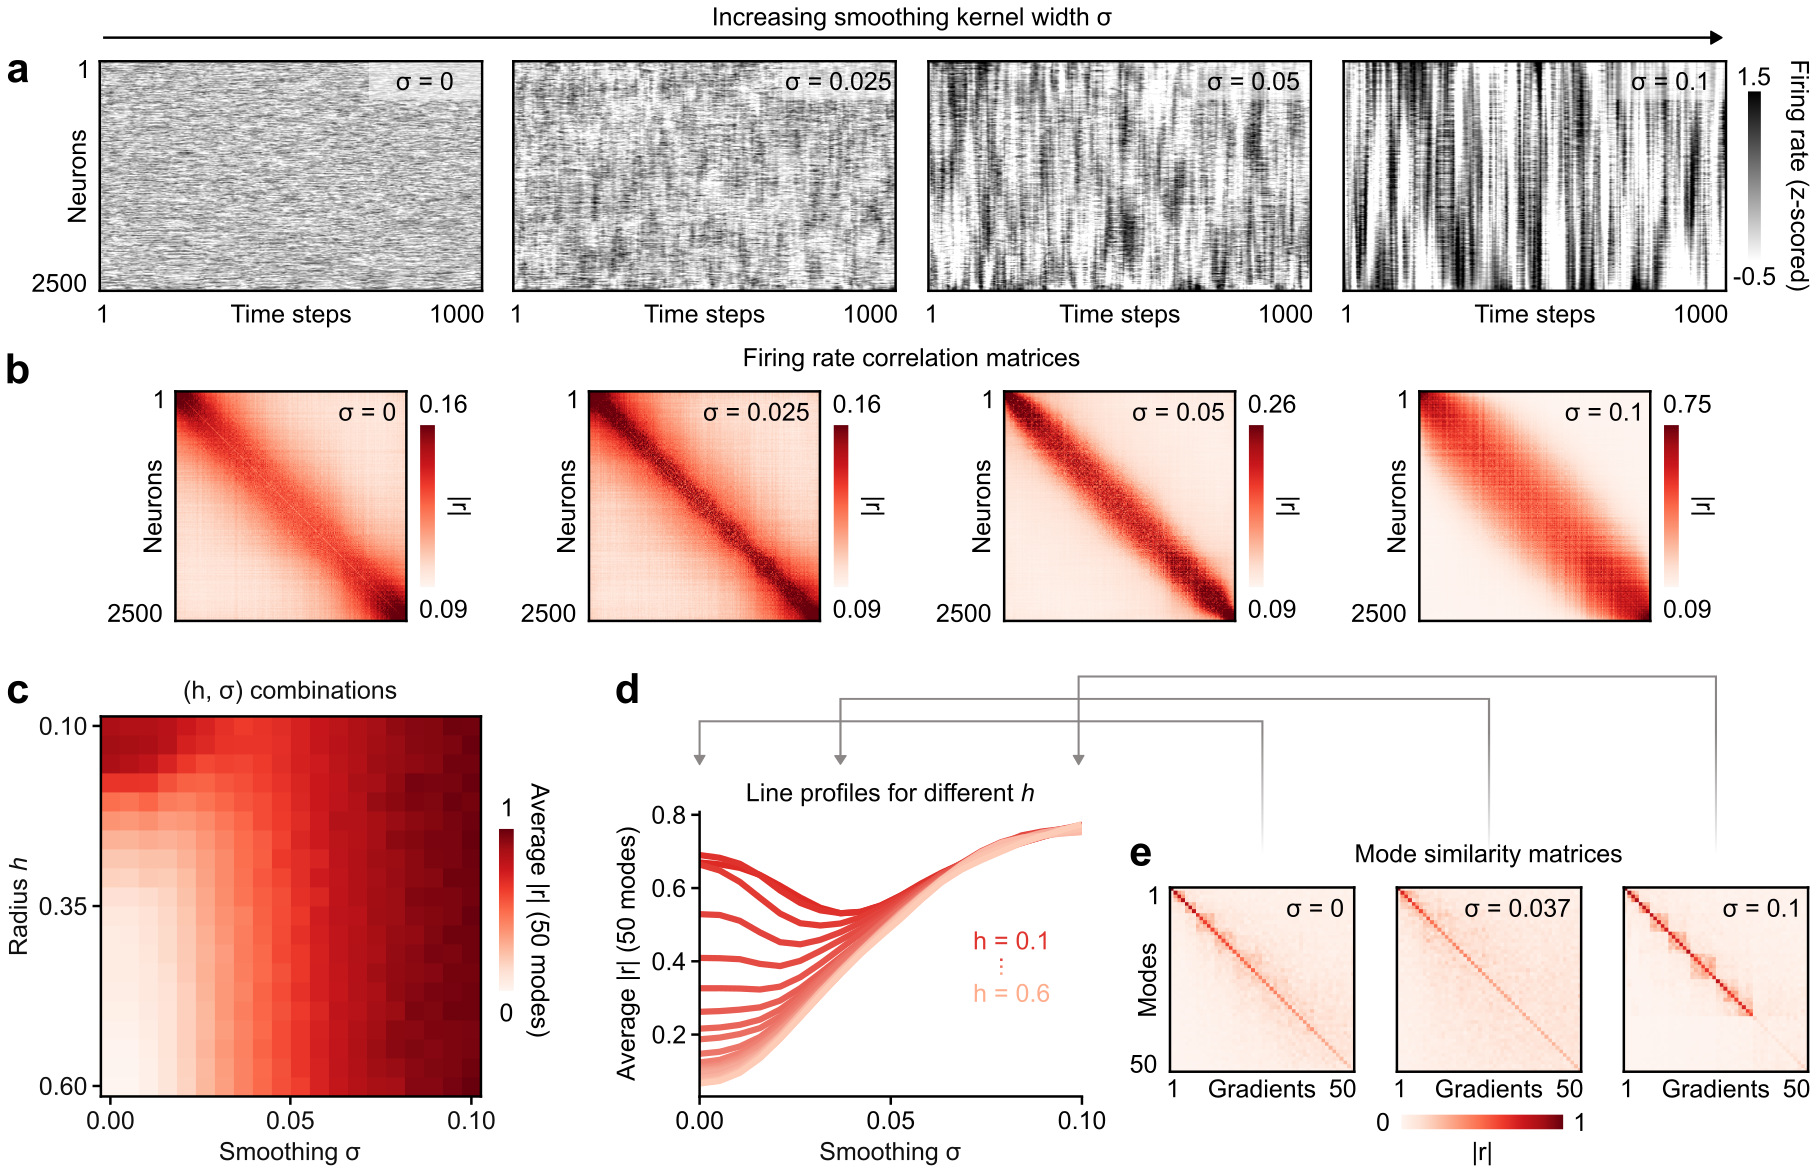
\includegraphics[width=1.0\linewidth]{figures/figure5.pdf}
    \caption{Differential effects of combined local connectivity and spatial filtering in numerical simulations. (\textbf{a}) Examples of simulated firing rate time series for increasing levels of spatial filtering (from left to right); neurons were sorted along the major axis of the ellipsoid to accentuate patterns. (\textbf{b}) Pairwise correlations of neuronal firing rates for increasing levels of spatial filtering, corresponding to the four time series of \textbf{a}; colors are scaled to the 5th and 95th percentiles of correlations to improve visualization. (\textbf{c}) Grid of eigenmode-gradient correlations averaged over 50 modes for different values of $h$ and $\sigma$; $N=1500$ neurons, 10 ellipsoid coordinate sets per pixel, with 100 averaged simulations per set. (\textbf{d}) Rows of the matrix of \textbf{c} (a mild gaussian smoothing has been applied to the curves to improve readability). (\textbf{e}) Eigenmode-gradient correlation matrices for $h=0.1$ and three different values of $\sigma$; the middle matrix corresponds to the case where filtering weakened the eigenmode-gradient correlations observed in the raw time series.}
    \label{fig5}
    \hrulefill
\end{figure*}

\subsection*{The larval zebrafish optic tectum exhibits geometric gradients}

\begin{figure*}[t]
    \centering
    \includegraphics[width=1.0\linewidth]{figures/figure6.pdf}
    \caption{The larval zebrafish optic tectum exhibits geometric gradients. (\textbf{a}) Schematization of the microscopy field of view. (\textbf{b}) Dimensions of the multi-plane imaging volume. (\textbf{c}) One example time-averaged calcium imaging plane, highlighting the nuclear-localized calcium sensor, as well as the periventricular layer (PVL) and neuropil regions of the tectum. (\textbf{d}) Example time series of PVL neurons in the right hemisphere from one animal, sorted using the Rastermap\cite{stringer2025rastermap} algorithm to accentuate patterns. (\textbf{e}) 3D visualization and anatomical contextualization of the right tectum volume, with tectal nodes used to subdivide the region and allow inter-individual comparisons. (\textbf{f}) Pairwise correlations of node activity, averaged across 12 animals; the matrix is sorted along the antero-posterior brain axis. (\textbf{g}) Correlation-distance relationship obtained from the previous matrix, Spearman's $r=-0.618$. (\textbf{h}) Top, first 7 eigenmodes of the right tectum; bottom, corresponding functional gradients derived from calcium activity correlations; red and blue colors represent arbitrary positive and negative values, respectively. (\textbf{i}) Correlation matrix of tectal eigenmode-gradient pairs; notice the diagonal disappearing after roughly 20 modes.}
    \label{fig6}
    \hrulefill
\end{figure*}

Our combined numerical analyses yield three testable hypotheses for experimental validation. First, homogeneous, locally connected, and correlated neuronal networks should exhibit geometric gradients. Second, if neuronal arborizations are spatially extended, there should be a detectable cutoff in the mapping between gradients and geometric eigenmodes. Third, the wavelength associated with this cutoff should correspond to the effective connectivity radius of neurons. To validate these hypotheses, we used volumetric two-photon microscopy and calcium imaging to record spontaneous neuronal activity in the optic tectum of zebrafish larvae at cellular resolution (Fig. \ref{fig6}\textbf{a}, Tg(\textit{elavl3}:H2B-GCaMP6s)\cite{vladimirov2014light}). The optic tectum is the main retinorecipient brain region of the zebrafish\cite{baier2024visual} and exhibits spontaneous bursts of spatially compact neuronal assemblies\cite{avitan2017spontaneous, marachlian2018principles}. This phenomenon is thought to arise from local recurrent excitatory connections between tectal interneurons\cite{zylbertal2023recurrent}, a feature analogous to the connectivity radius in our simulations.

We recorded 10 minutes of activity from thousands of neurons distributed throughout the entire tectal volume (15 imaging planes at $\approx2$ Hz, $n=12$ larvae, Fig. \ref{fig6}\textbf{b}, Methods). We focused our analysis on cells within the periventricular layer (PVL neurons, Fig. \ref{fig6}\textbf{c}), a continuous and anatomically delineated structure. To avoid potential discontinuities across the midline, we restricted our analysis to the right hemisphere ($2845\pm578$ neurons), but similar results were obtained from the other hemisphere. Most neurons displayed low-amplitude calcium fluctuations punctuated by occasional large-amplitude transients involving tens to hundreds of neurons (Fig. \ref{fig6}\textbf{d}, Supp. Video 2). To average correlations across individuals, we used non-rigid registration of anatomical volumes\cite{avants2009advanced} to project all neurons to a common atlas coordinate system (mapZebrain atlas\cite{kunst2019cellular}, Methods), then subdivided the right hemisphere tectum mask into 400 nodes of roughly equal size to which we then assigned individual neurons (Fig. \ref{fig6}\textbf{e}, 397 nodes following exclusion criteria, Methods). We computed the time series by averaging single-neuron activity ($7.16\pm4.35$ neurons per node), and then computed the pairwise tectal correlations (Fig. \ref{fig6}\textbf{f}). As previously reported\cite{zylbertal2023recurrent}, we observed a strong distance-dependent decay in correlation strength within the region (Fig. \ref{fig6}\textbf{f}, Spearman $r=-0.618$), with correlations reaching their baseline level beyond roughly $100$ microns. 

Next, we calculated functional gradients from the group-averaged correlations and compared them to geometric eigenmodes of the tectum’s 3D shape (Fig. \ref{fig6}\textbf{h}, Methods). We observed positive correlations between eigenmodes and gradients across roughly the first 20 modes, beyond which the correspondence vanished (Fig. \ref{fig6}\textbf{i}). We validated the significance of this correspondence by benchmarking against null correlations obtained by spatially shuffling the eigenmode ensembles ($P<0.01$, $1000$ variogram-preserving permutation sets\cite{burt2020generative}, Methods). We also excluded the possibility that high correlations resulted from spatial downsampling, as the eigenmode-gradient correlations were nearly identical across varying coarse-graining levels (Supp. Fig. \ref{supp_coarsegraining}\textbf{a}). At the individual fish level, however, tectal correlations exhibited variability (Supp. Fig. \ref{supp_coarsegraining}\textbf{b}) and eigenmode-gradient correlations were weaker (Supp. Fig. \ref{supp_coarsegraining}\textbf{c}), likely reflecting the limited statistical power of short duration recordings to properly sample the correlation structure of the tectum.

These results demonstrate that the functional organization of the optic tectum is tightly coupled to its geometry, up to a cutoff point where the correspondence vanishes, thus validating our first two hypotheses raised from numerical simulations. Most importantly, these findings replicate observations made by Pang et al in human subcortical structures\cite{pang2023geometric}, further extending them to a much smaller brain structure at cellular resolution in zebrafish larvae.

\subsection*{The geometric cutoff point predicts the size of tectal arbors}

\begin{figure*}[t]
    \centering
    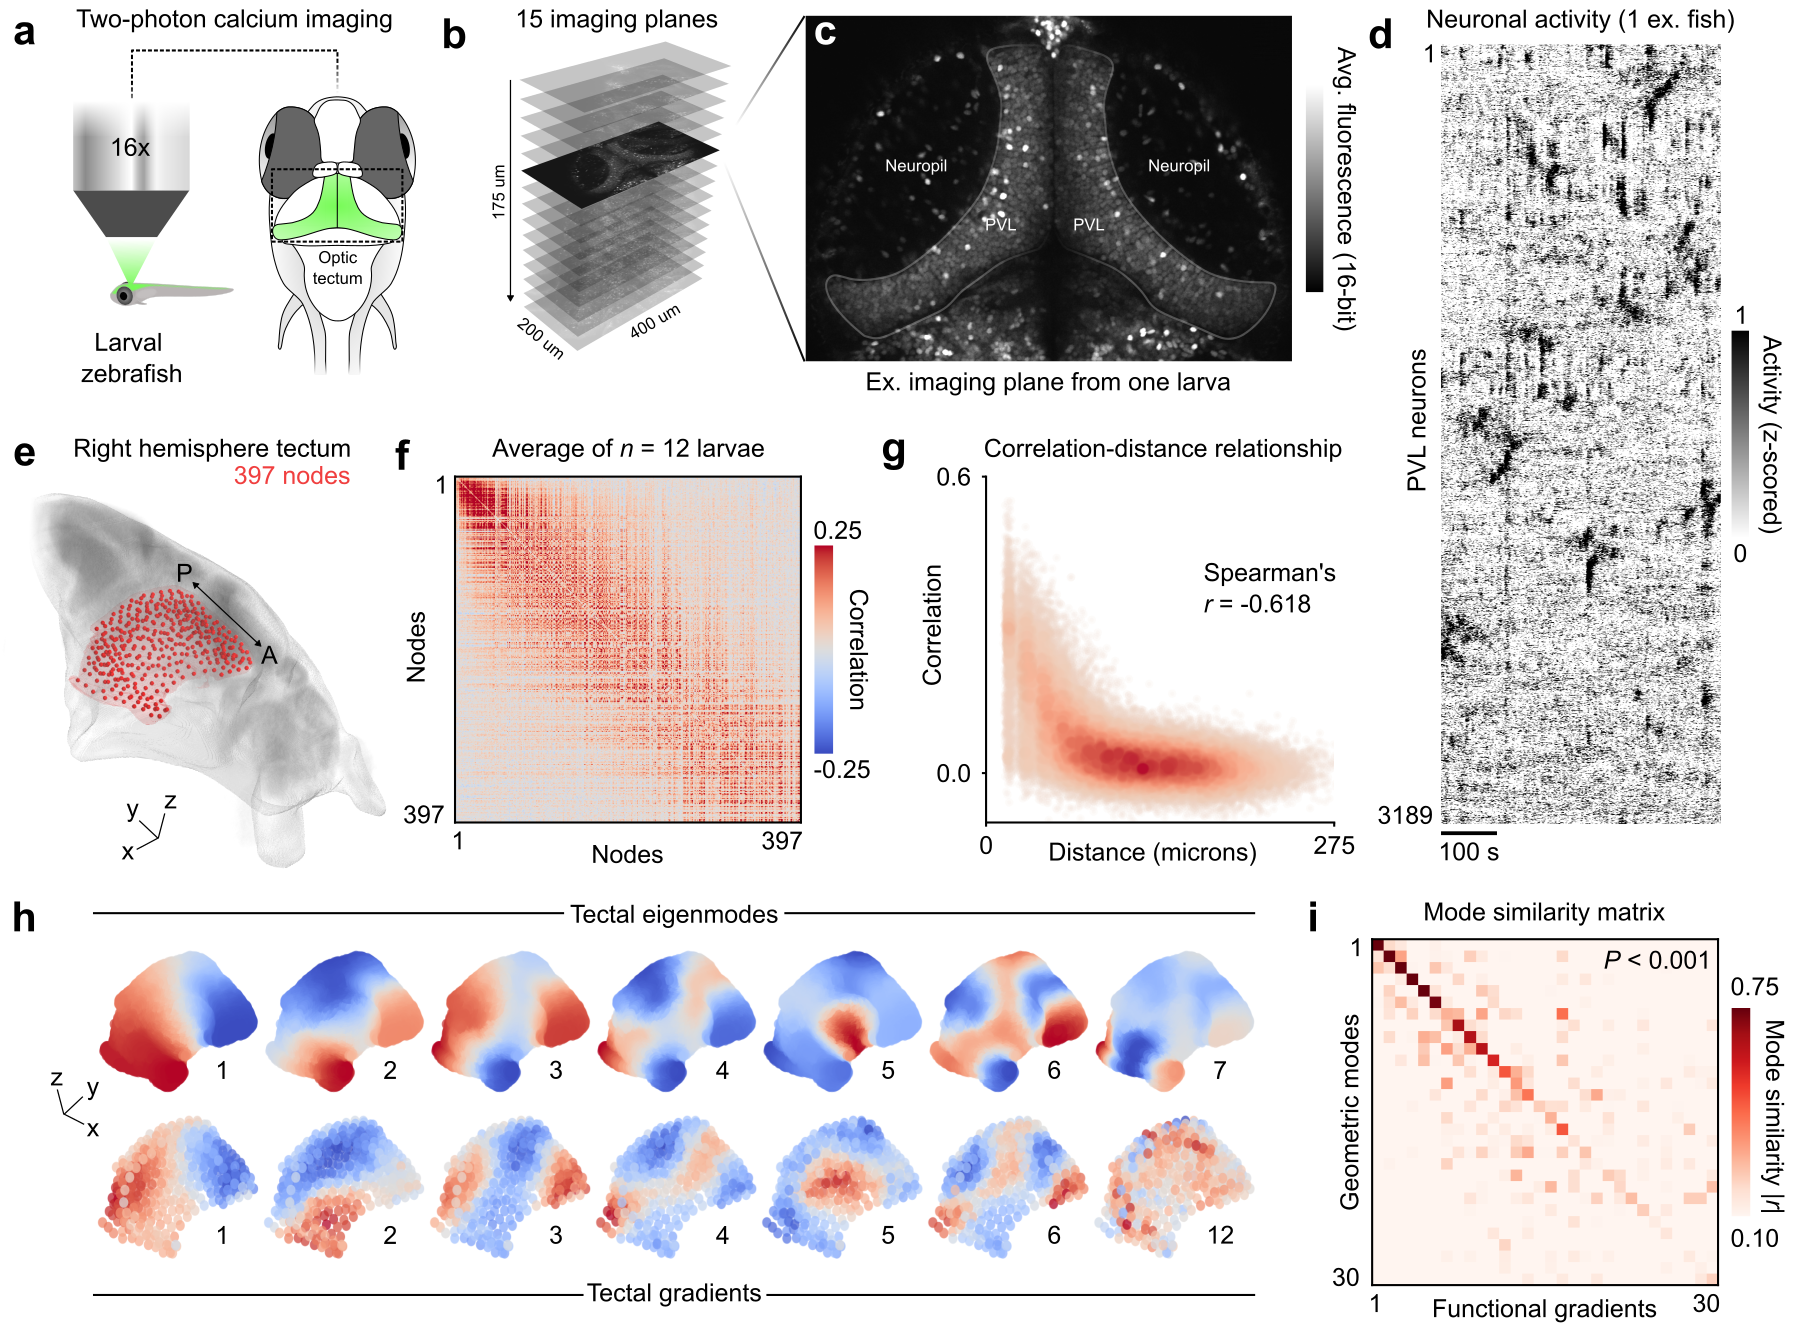
\includegraphics[width=1.0\linewidth]{figures/figure7.pdf}
    \caption{Arbor sizes of tectal neurons are consistent with the predicted connectivity radius. (\textbf{a}) Top view of 525 tectal neuron morphologies, colored by the antero-posterior location of the cell body, accentuating the topographic organization of neurites within the adjacent neuropil. (\textbf{b}) Example morphologies of 18 neurons, visualized from above. (\textbf{c}) Piecewise-linear regression of tectal eigenmode-gradient correlations to identify a cutoff point, corresponding to eigenmode 20. (\textbf{d}) Schematization of the first connectivity radius estimation method; the 95th percentile of terminal distances (relative to the arbor center of mass) is doubled to estimate the radius. (\textbf{e}) Distribution of connectivity radii obtained from method 1; the red line indicates the predicted radius from the geometric cutoff point, while the black line is the distribution mean; the pink shaded region represents the 95\% confidence interval of the estimated radius, based on the linear relationship in Supp. Fig. \ref{supp_tectum_cutoff}\textbf{d}. (\textbf{f}) Schematization of the second connectivity radius estimation method; pseudo-connections are identified from neighboring terminals, then the 95th percentile of soma-soma distances is identified for each neuron. (\textbf{g}) Distribution of connectivity radii obtained from method 2; the red line indicates the predicted radius from the geometric cutoff point, while the black line is the distribution mean; the pink shaded region represents the 95\% confidence interval of the estimated radius.}
    \label{fig7}
    \hrulefill
\end{figure*}

The cutoff point observed in the eigenmode-gradient correspondence suggests that the connectivity radius of neurons in the optic tectum is non-negligible, relative to the region's overall size. To characterize the underlying connectivity structure, we used a single-neuron morphological dataset from the mapZebrain atlas\cite{kunst2019cellular} to analyze the arborescence of 525 independently reconstructed tectal neurons (Fig. \ref{fig7}\textbf{a}). Unlike the radially extended connections used in our simulations, tectal interneurons extend both dendritic and axonal processes into an adjacent neuropil region\cite{robles2011characterization} (Fig. \textbf{a}). While a subset of neurons projects to the contralateral tectum or downstream hindbrain motor targets\cite{helmbrecht2018topography}, many arbors are confined entirely within the ipsilateral tectal neuropil (Fig. \ref{fig7}\textbf{b}, 18 example morphologies, top view). 

We first identified the cutoff eigenmode from the diagonal of the eigenmode-gradient correlation matrix (Fig. \ref{fig6}\textbf{i}) by fitting a piece-wise linear regression with a variable elbow point (Fig. \ref{fig7}\textbf{c}, $R^2=0.874$). Although this approach differs from the one used previously in Fig. \ref{fig3}, we validated its ability to recover the connectivity radius $h$ of simulated networks within tectal geometry ($R^2=0.955$, Supp. Fig. \ref{supp_tectum_cutoff}). In experimental data, the estimated cutoff was observed at eigenmode 20, corresponding to a spatial wavelength of $\lambda=127.12$ $\mu$m, which predicts a connectivity radius of $52.04$ $\mu$m between tectal neurons when inverting the linear relationship in Supp. Fig. \ref{supp_tectum_cutoff}. 

To validate this prediction, we analyzed tectal neuron morphologies using two complementary approaches. First, we estimated arbor radii by measuring the spatial extent of each neuron's neurite terminals contained within the tectum neuropil (Methods), then multiplied the estimated radii by two to approximate the effective connectivity radius for each neuron (Fig. \ref{fig7}\textbf{d}). This simple geometric method assumes that synaptic contacts arise from overlapping neurite clouds. The resulting distribution of connectivity radii had a median radius of $54.01$ $\mu$m, corresponding to a $3.6\%$ deviation from the eigenmode-based estimate (Fig. \ref{fig7}\textbf{e}). In the second approach, we identified pseudo-connections between pairs of neurons by detecting at least one pair of terminals located within 5 $\mu$m of each other (Fig. \ref{fig7}\textbf{f}, Methods). For each neuron, we then estimated the connectivity radius as a certain percentile of soma-soma distances among its pseudo-connected partners. This yielded a distribution with a median of $54.37$ $\mu$m, within $4.3\%$ of the predicted radius (Fig. \ref{fig7}\textbf{g}). Compared to the first method, this approach more directly captures the anisotropic geometry of tectal arbors, including their tendency to innervate different parallel neuropil layers. Although noise in the functional data could in principle influence the observed cutoff point, we confirmed that the estimated cutoff wavelength remains stable across a broad range of simulated noise levels (up to 3 data standard deviations in additive noise, Supp. Fig. \ref{supp_noise}). Therefore, the cutoff point most likely reflects the intrinsic spatial scale of connectivity within the tectum.

Overall, both morphological analyzes yielded connectivity radius estimates that closely matched the value predicted from the cutoff point of geometric gradients. These results provide converging evidence from functional and structural datasets to support our third hypothesis: the geometric cutoff point in the eigenmode-gradient correspondence reflects the spatial extent of neuronal connectivity.

\subsection*{Whole-brain functional connectivity gradients do not reflect geometry}

Lastly, we examined the impact of spatial filtering on FC gradients in experimental data. Using our previous whole-brain two-photon calcium imaging dataset\cite{legare2025structural}, we computed whole-brain FC gradients ($n=22$ larvae, Methods). Given the heterogeneous structural connectivity and numerous long-range projections found in the brain, we expected weak correspondence between eigenmodes and gradients in the absence of spatial filtering at brain-wide scale. To verify this hypothesis, we first mapped individual neurons into 987 uniformly sized and non-overlapping nodes per brain hemisphere, then averaged single-neuron calcium fluorescence within each node before computing pairwise correlations, averaging correlation matrices across both hemispheres and animals (Supp. Fig. \ref{supp_wholebrain}\textbf{b}, Methods). Brain-wide correlations exhibited a weak decay with distance, relative to the comparatively stronger decay observed within the optic tectum (Spearman's $r=-0.298$, Supp. Fig. \ref{supp_wholebrain}\textbf{c}). Next, we segmented the external boundary of the brain to define a volumetric domain for eigenmode calculation, treating the brain as a single homogeneous structure without accounting for internal anatomical boundaries (Methods). We computed both single- and bi-hemispheric eigenmodes and compared them with single-hemisphere functional gradients (Supp. Fig. \ref{supp_wholebrain}\textbf{d}). Without spatial filtering, we observed small but significant correlations between gradients and eigenmodes (Supp. Fig. \ref{supp_wholebrain}\textbf{e}, $P<0.005$, 1000 variogram-preserving spatial permutations, Methods). Thus, brain-wide correlations are weakly constrained by geometry, presumably due to the high heterogeneity of the larval brain volume.

Next, we progressively applied spatial filtering to single-neuron activity, which drove high local correlations and resulted in a marked increase of the average eigenmode-gradient correlations (Supp. Fig. \ref{supp_smoothing}\textbf{a}-\textbf{b}). A similar positive effect was observed when spatial filtering was applied to tectal data (Supp. Fig. \ref{supp_smoothing}\textbf{a}-\textbf{b}). Despite different levels of homogeneity and local connectivity, spatial filtering in both geometries consistently strengthened the correspondence between eigenmodes and gradients, in contrast with the heterogeneous and sometimes detrimental effects of filtering observed in numerical simulations (Fig. \ref{fig5}). Peak correlations between eigenmodes and gradients were obtained at relatively large kernel widths of 50 and 18 microns for the whole-brain and the optic tectum respectively (Supp. Fig. \ref{supp_smoothing}\textbf{b}), representing around $7\%$ of each system's characteristic length (740 microns for the whole brain, and 260 microns for a single tectal hemisphere). Although spatial filtering monotonously increased the eigenmode-gradient correlations, the predicted connectivity radius of the optic tectum, inferred using piecewise linear fits as previously, remained largely unchanged (Supp. Fig. \ref{supp_smoothing}\textbf{c}). Thus, spatial filtering may inflate the eigenmode-gradient correlations in real data, but its peak effect is observed at unreasonably large spatial kernels, without considerably altering the inferred connectivity radius.

Overall, these results suggest that, while spatial filtering could artificially drive geometric gradients in calcium imaging data where no such feature is initially present, more conservative filtering does not considerably increase eigenmode-gradient correlations, nor does it bias other derived measures such as the predicted connectivity radius of the system.

\section*{Discussion}

% Discuss which structures should exhibit geometric gradients
% and why deviations from the geometric regime are interesting
% (for instance, cortical eigenmodes do not reflect gradients, which could indicate
% that widespread coactivation patterns could take over the local correlations)
% Discuss 

The influence of geometry on nervous system organization is well established, with brain functions organized along gyri and sulci of the neocortex\cite{petersen2024principles}. The prevalence of short-range connections in both small\cite{kunst2019cellular} and large nervous systems\cite{ercsey2013predictive} supports dynamical processes like localized population bursts and wave propagation, and under certain approximations, long-range connections may exert only a secondary influence to short-range ones\cite{robinson1997propagation}. Such approximations imply that neural dynamics are fundamentally shaped by geometry in ways that are not fully captured by classical connectivity measures\cite{robinson2016eigenmodes, pang2023geometric}. Whether connectivity or geometry provide greater explanatory power over the brain's complex spatiotemporal dynamics has recently been debated\cite{pang2023geometric, faskowitz2023commentary, pang2023reply, vohryzek2025human}.

Here, we adopted a generative modeling approach by simulating network dynamics in various geometries to explore how geometric constraints shape emergent functional patterns in brain networks. Specifically, we investigated recent findings from Pang and colleagues who reported striking similarities between FC gradients and geometric eigenmodes in human subcortical structures\cite{pang2023geometric}. To elucidate this alignment in different geometries, we imposed a singular constraint on simulations: that neurons are connected to all their neighbors within a certain radius. Regardless of the dynamical model or spatial embedding, the resulting dynamics exhibited local correlations, yielding connectivity gradients that strongly resembled geometric eigenmodes. This outcome aligns with previous theoretical predictions: as network connections become increasingly local, geometry imprints itself onto the network’s structure\cite{belkin2008towards, GarcaTrillos2019}. Consequently, eigenvectors of the graph Laplacian, a measure of random diffusion akin to connectivity gradients, converge toward those of the LBO derived from the graph's spatial embedding. Despite slight mathematical differences, we observed a similar spectral convergence between across multiple gradient derivation methodologies. While the formal relationship between these operators remains to be fully elucidated, our findings suggest that geometric gradients emerge naturally when local connections and correlations are dominant features. Importantly, by constraining structural connections with geometry, our modeling results argue for a more nuanced picture where geometry, connectivity, and function are all interwoven.

A critical insight from our results is that geometric gradients do not arise solely from wave propagation, as they persist across diverse dynamical systems that do not explicitly implement or exhibit waves. Nevertheless, homogeneous wave-like dynamics are expected to yield geometric gradients due to the local correlations they induce\cite{ackman2012retinal}. The emergence of geometric gradients from various generative mechanisms and dynamical systems, however, highlights an important limitation of gradients derived from simple pairwise statistics, which can conflate diverse dynamical processes into similar spatial patterns. The choice of pairwise statistic to evaluate functional interactions remains an arbitrary methodological choice in neuroimaging studies, and diffusion maps applied to other pairwise interaction matrices might reveal different spatial patterns that do not reflect geometry, especially when using metrics that correlate less with spatial distance\cite{liu2024benchmarking}. Given the limitations of linear correlations and the limited spatial resolution of MRI, it is unclear if the geometric gradients observed by Pang and colleagues\cite{pang2023geometric} in the hippocampus, striatum and thalamus reflect wave dynamics, highly localized population bursts, or filtering artifacts. Traveling waves have been observed in the hippocampus using electrophysiological approaches\cite{lubenov2009hippocampal, patel2012traveling}, and cortical waves can be decoded from subcortical activity in striatum and thalamus using neuropixels probes\cite{ye2023brain}. Therefore, all three regions could plausibly support topographically organized activity patterns that translate into geometric functional gradients in macroscopic observations. Given the possibly ambiguous effects of spatial filtering, it is difficult to assess how previous fMRI-derived results might have been biased, and subsequent efforts are required to better understand what separates intrinsic from filtering-induced correlations in human neuroimaging data. Nevertheless, we observed generally mild effects in experimental data when spatial filtering kernel sizes were conservatively small, especially when a system did not exhibit geometric gradients in the first place. Beyond these methodological considerations, our study provides an example of how temporally static statistical patterns such as FC gradients can be agnostic to the nature of underlying dynamical processes, and should therefore be combined with other complementary methods to more aptly identify their dynamical origins.

Our simulations further reveal that geometric gradients are robust to heterogeneities and long-range connections. Even when 10–20\% of network connections were randomized, the correspondence between functional gradients and geometric eigenmodes remained largely intact, suggesting that this phenomenon is robust to heterogeneous biological conditions. Although theoretical results show that perfect correspondence between gradients and eigenmodes occurs only in the limit of infinitesimally local connectivity\cite{GarcaTrillos2019}, real neurons extend arbors beyond their immediate neighbors. As shown in our simulations, spatially extended connectivity causes the geometric mapping between eigenmodes and gradients to break beyond a specific eigenmode wavelength that reflects the size of underlying arbors. We experimentally validated this phenomenon using two-photon imaging in the larval zebrafish optic tectum, a locally connected structure with localized bursting activity\cite{avitan2017spontaneous}. As expected, we observed a good correspondence between eigenmodes and gradients in this region, and further observed a geometric cutoff point that was not a trivial consequence of noise. Rather, this cutoff point quantitatively reflected the median size of tectal neuronal arbors. While the optic tectum is not entirely homogeneous---featuring local connectivity variations and a layered cell-type organization\cite{helmbrecht2018topography, shainer2025transcriptomic}---its connections remain predominantly local, reflecting the visuotopic arrangement of tectal neurons\cite{niell2005functional, li2022topographic}. The well-documented compact bursting phenomenon in this region yields exponentially decaying correlations\cite{zylbertal2023recurrent}, a sufficient condition for the emergence of geometric gradients. Our results extend the findings of Pang and colleagues\cite{pang2023geometric} to a small vertebrate brain structure at cellular resolution, where activity signals are well-resolved, non-overlapping, and do not require spatial filtering. This contributes to a recent line of work demonstrating the value of whole-brain functional imaging in zebrafish larvae as a strategic model for comparative systems neuroscience\cite{legare2025structural}. Despite vast differences in brain size and complexity between mammals and smaller vertebrates or invertebrates, core principles of brain structure and function often generalize and can be experimentally dissected in small model organisms at cellular resolution\cite{ahrens2013whole, lin2022imaging}. Translating insights from human neuroimaging into experimentally tractable animal models is an essential step toward the validation of observations or theories established at macroscopic scales.

Despite experimental validation, our work lacks a formal theoretical framework that links network dynamics to geometric gradients or relates arbor size to cutoff eigenmode wavelengths, instead relying on linear regressions derived from simulations. Further theoretical efforts are needed to clarify how geometry constrains structural connections---via factors such as physicality\cite{posfai2024impact} or wiring cost minimization\cite{bullmore2012economy}---and how structural connections drive geometric features in neuronal dynamics. In this view, the influence of geometry on brain function is not direct but mediated through the structure function relationship of brain networks as a crucial intermediary\cite{suarez2020linking, fotiadis2024structure}. Beyond synaptic connectivity, other biophysical processes such as extracellular neurotransmitter diffusion\cite{randi2023neural} and gap junction-mediated synchronization\cite{ponce2018whole} also contribute to localized network dynamics. Exploring these alternative signaling mechanisms could offer a richer understanding of how brain function is grounded in physical space. As brain morphology varies across species, development, and pathology\cite{thompson2004mapping}, understanding the influence of geometry on neuronal activity\cite{pang2023geometric} and brain organization\cite{pang2025geometric} is of both fundamental and translational interest. Our findings reinforce the central role of short-range interactions---a hallmark of brain networks and many other physical systems---as important drivers of geometric functional features in three-dimensional nervous systems.

\section*{Methods}

\subsection*{Geometric eigenmodes}

Geometric eigenmodes are the solutions to the Laplace-Beltrami eigenvalue problem defined on a Riemannian manifold, a type of geometric space where distance and curvature are locally defined. Mathematically, they are functions $\phi_k$ on that manifold, indexed by $k\in \mathbb{N}$, that satisfy $\Delta \phi_k=\lambda_k\phi_k$, where $\Delta$ is the Laplace-Beltrami operator, $\lambda_k$ are the corresponding eigenvalues, with $\lambda_k$ increasing with $k$. The set of all $\phi_k$ forms an orthonormal basis of square-integrable functions over the manifold, ordered by increasing spatial frequency, i.e., lower-indexed modes correspond to smoother, slowly varying patterns, while higher-indexed modes exhibit finer spatial structure and more rapid oscillations. These eigenmodes represent intrinsic spatial harmonics of the geometric space and are commonly used to model patterns of diffusion or vibration constrained by geometry. 

To derive the geometric eigenmodes of each geometry---that is, each three-dimensional Riemannian manifold---, we first generated volumetric tetrahedral mesh representations using the pygalmesh Python package. This process yielded approximately 30,000–40,000 tetrahedron vertices uniformly distributed throughout each volume and bounded within a unit cube ($x\in[0,1]$), such that a distance of 1 represents a characteristic length scale common to all geometries considered. We then computed the geometric eigenmodes using a finite elements method (FEM) implemented in the LaPy package, solving for the first 100 eigenfunctions of the Laplace-Beltrami operator for each mesh, excluding the first constant eigenmode. The resulting eigenmodes are spatial functions defined over the mesh vertices, ordered by their eigenvalues (spatial wavelengths), with the first eigenmode corresponding to the smoothest pattern (longest wavelength) and higher-order eigenmodes representing increasingly fine-grained spatial variations (smallest wavelength).

\subsection*{Simulations of neuronal activity}

We simulated various dynamical models of neurons (described in the following section) embedded within 3D geometries. Although each model involved different parameters, all simulations followed a similar standardized protocol. Neuron coordinates were first randomly sampled from the set of vertices generated during the tetrahedral mesh construction described earlier. A binary connectivity matrix $W^{\text{bin}}$ was then generated by connecting nearby neurons such that $W^{\text{bin}}_{ij}=1$ if $d_{ij} < h$ and $W^{\text{bin}}_{ij}=0$ if $d_{ij} \geq h$, where $h$ is the connectivity radius parameters and $d_{ij}$ is the euclidean distance that separates neurons $i$ and $j$. Note that this binary network definition corresponds to a random geometric network model\cite{penrose2003random}. Next, $W^{\text{bin}}$ was transformed into a directed, weighted matrix $W$ whose nonzero values were drawn from different distributions specific to each dynamical model, ensuring dynamics that are bounded, sustained, and exhibit rich, possibly chaotic behavior. Neuronal firing rates were then generated by numerically integrating the system over $T=250$ to $1000$ time steps using Euler's method. To quantify emergent functional relationships between neurons, an average correlation matrix $C$ whose elements are the absolute pairwise Pearson correlation coefficients of neuronal firing rates averaged over 100 independent simulations. In each run, the connectivity weights and initial conditions were reinitialized, while the neuron positions---and therefore the binary structure $W^{\text{bin}}$---remained fixed. This ensured a representative sampling of possible dynamics unfolding on the same geometric scaffold. We used absolute correlations to capture both large positive and negative relationships between neurons, though in practice, the largest-magnitude correlations were predominantly positive and similar results could be achieved without taking the absolute value, either by normalizing or clipping negative values. Finally, the resulting average correlation matrix $C$ was used for subsequent gradient analysis. For some analyses, we repeated the entire simulation protocol 10 times per geometry and parameterization---each time resampling node coordinates, constructing a new connectivity graph, simulating dynamics, and averaging correlations---to reduce bias introduced by the randomized node coordinates and to suppress noise in the eigenmode-gradient correlations. All numerical simulations were implemented in \verb|PyTorch| using \verb|CUDA|, enabling efficient GPU parallelization and substantially accelerating the numerical integration.

\subsection*{Dynamical models}

\subsubsection*{Model \#1: Chaotic firing rate network}

For the first and main dynamical model used throughout most of the study, we simulated spontaneous firing rate dynamics---also known as the graded response model--- from the following equations\cite{gerstner1995time}:
\begin{align*}
    \tau\frac{d\textbf{x}}{dt}=-\textbf{x} + g\textbf{W}\textbf{r},\\
    \textbf{r}=\tanh{(\textbf{x})},
\end{align*}
where $\textbf{x}(t)\in \mathbb{R}^N$ describes an internal variable for each neuron at time $t$, analogous to a membrane potential, while $\textbf{r}(t)$ is the vector of firing rates at time $t$ obtained through a nonlinearity $\tanh (\textbf{x})$, with $\tanh$ applied element-wise. The parameter $\tau$ dictates the time constant of neurons, and $g$ is the network coupling strength, which brings the dynamics into a chaotic regime for $g>1$ in the thermodynamic limit \cite{sompolinsky1988chaos}. The connectivity matrix $W \in \mathbb{R}^{N \times N}$ has entries drawn independently and identically from a normal distribution $\mathcal{N}\left(0, \frac{1}{\sqrt{N\rho}}\right)$, with positive and negative values interpreted as excitatory and inhibitory synaptic weights, respectively. The parameter $\rho$ reflects the empirical average connection density, whose exact value fluctuates with node coordinates and connectivity radius $h$ (networks with small $h$ are sparser, and vice-versa). Crucially, the $\rho$ normalization of connection weights ensures that the overall strength of inputs to each neuron remains constant as the connectivity radius $h$ increases, preventing runaway activity in denser network configurations. We used a stronger coupling of $g=3$ to compensate for network sparsity and to ensure rich chaotic activity time series (Fig. \ref{fig1}\textbf{c}). We used a small time constant of $\tau=3$ to produce faster dynamics and reduce the overall integration time required to properly sample the correlations. Initial conditions $\textbf{x}(0)$ were sampled randomly and uniformly in the range $[-1, 1]$ before numerically integrating the system.

\subsubsection*{Model \#2: Chaotic firing rate network + Dale's law}

For the second dynamical model, we adapted the first dynamical model by changing the neuronal activation function and applying Dale's law to the connectivity matrix. Instead of the standard $\textbf{r}=\tanh(\textbf{x})$, which varies between $-1$ and $1$, we used a strictly positive activation function defined in a previous study,
$$
\textbf{r}(\textbf{x})=
\begin{cases}
r_0\tanh(\textbf{x}/r_0) & \text{for } x\leq0\\
(2-r_0)\tanh(\textbf{x}/(2-r_0)) & \text{for } x>0,
\end{cases}
$$
with firing rates ranging $\textbf{r}(t)$ from 0 to 2. The $r_0$ parameter represents a fixed background firing rate, which we set to $r_0=0.1$. Note that for $r_0=1$, this function reduces to the standard $\tanh$ function. In addition to this change in the neuron dynamics, we applied Dale's law, that is, we imposed strictly positive or negative signs on the columns of $W$. This ensures that each neuron's outputs are strictly excitatory or inbibitory, respectively. We used a $1:1$ ratio of excitatory and inhibitory neurons to maintain properly balanced oscillatory dynamics. These combined changes to the network architecture led to qualitatively different activity, with large spatially patterned population fluctuations that were not present in the more chaotic dynamics of model \#1. Despite these differences, both models produced spatially decaying correlations and comparable geometric gradients (Supp. Fig. \ref{supp_dynamics}).

\subsubsection*{Model \#3: Kuramoto-Sakaguchi oscillators}

For the third dynamical model, we considered a network of $N$ coupled Kuramoto-Sakaguchi oscillators, each interpreted as a neuron, such that the phase $\theta_i$ of neuron $i$ evolves according to \cite{sakaguchi1986soluble}
$$
    \tau\frac{d\theta_i}{dt}=\omega_i+ \frac{g}{N}\sum_{j=1}^N W_{ij}\sin(\theta_j - \theta_i - \alpha_{ij}),
$$
where $\tau$ is a global time constant, $\omega_i$ is the natural frequency of neuron $i$, $W$ is the connectivity matrix, $g$ is a global coupling strength parameter, and $\alpha_{ij}$ is a phase-lag parameter. For this model, the weights in $W$ remained binary, with $W_{ij} = 1$ indicating the presence of a connection from neuron $j$ to neuron $i$, and $W_{ij} = 0$ otherwise. The phase lag matrix $\alpha$ was obtained by multiplying the euclidean distance matrix by an arbitrary scaling parameter of $50$ to mimick propagation delays along structural connections of variable lengths\cite{fukushima2018comparison}. This distance-dependent phase lag approximates propagation delays and aims to maintain the network in a chaotic regime. We set $g=2000$, $\tau=100$, and we randomly sampled natural frequencies according to $\omega \sim \mathcal{N}(2, 0.1)$. Phases were initialized randomly and uniformly in the $[0, 2\pi]$ range. Parameter values were selected by a linear sweep to maximize the alignment between geometric eigenmodes and FC gradients.

\subsubsection*{Model \#4: Binary stochastic neurons}

For the fourth dynamical model, we implemented a simple binary stochastic neuronal network where the $N$-dimensional network state vector $\textbf{x}$ is binary, with ones representing active neurons and zeros representing inactive neurons. This model can be viewed as a Cowan-type Markov chain model of neurons \cite{painchaud2022beyond, murphy2024duality} with a clipped ReLU activation function. More explicitly, the state evolution is governed by two parameters: $P_a$, the probability that a neuron becomes active per active presynaptic neuron, and $P_d$, the probability that a neuron becomes inactive spontaneously at each integration step. For this model, connectivity matrix $W$ remained binary, and Dale's law was applied in a $1:1$ ratio to ensure balanced excitatory and inhibitory interactions. At each time step, inputs from active neurons were summed at each postsynaptic neuron, then the resulting integer number of inputs was multiplied by $P_a$ to yield an activation probability, which we clipped in the range $[0, 1]$. Importantly, for a sufficient number of positive inputs, postsynaptic neurons are guaranteed to become active. We initialized the network with roughly $10\%$ of active neurons, and used $P_a=0.15$ and $P_d=0.5$ to obtain sustained chaotic dynamics.

\subsubsection*{Model \#5: Spiking neurons + calcium dynamics}

For the fifth and final dynamical model, we implemented a discrete-time version of a conductance-based leaky integrate-and-fire (LIF) neuronal network \cite{izhikevich2007dynamical} with simplified calcium dynamics. The network consists of $N_E$ excitatory neurons and $N_I$ inhibitory neurons, whose membrane potentials and synaptic conductances evolve according to
\vspace{-0.25cm}
\setlength{\jot}{4pt} % default is around 6pt
\begin{align*}
V_{E,i}(t+\Delta t) &= V_{E,i}(t)+\Delta t \Big(g_L(E_L-V_{E,i}(t)) + I_{E, i}(t) + g_{EE,i}(t)(E_E - V_{E,i}(t)) + g_{EI,i}(t)(E_I - V_{E,i}(t))\Big), \\
&\quad V_{E,i}(t)<V_{\text{thresh}}, \\
V_{E,i}(t+\Delta t) &= V_{\text{reset}}, \quad V_{E,i}(t)\geq V_{\text{thresh}}, \\
V_{I,i}(t+\Delta t) &= V_{I,i}(t)+\Delta t \Big(g_L(E_L-V_{E,i}(t)) + I_{I, i}(t) + g_{II,i}(t)(E_I - V_{I,i}(t)) + g_{IE,i}(t)(E_E - V_{I,i}(t))\Big), \\
&\quad V_{I,i}(t)<V_{\text{thresh}}, \\
V_{I,i}(t+\Delta t) &= V_{\text{reset}}, \quad V_{I,i}(t)\geq V_{\text{thresh}}, \\
g_{EE,i}(t + \Delta t) &= g_{EE,i}(t)\Big(1-\frac{\Delta t}{\tau}\Big) + \sum_{j=1}^{N_{E}}c_{EE,i,j}\delta_{E,j}(t), \\
g_{EI,i}(t + \Delta t) &= g_{EI,i}(t)\Big(1-\frac{\Delta t}{\tau}\Big) + \sum_{j=1}^{N_{I}}c_{EI,i,j}\delta_{I,j}(t), \\
g_{II,i}(t + \Delta t) &= g_{II,i}(t)\Big(1-\frac{\Delta t}{\tau}\Big) + \sum_{j=1}^{N_{I}}c_{II,i,j}\delta_{I,j}(t), \\
g_{IE,i}(t + \Delta t) &= g_{IE,i}(t)\Big(1-\frac{\Delta t}{\tau}\Big) + \sum_{j=1}^{N_{E}}c_{IE,i,j}\delta_{E,j}(t).
\end{align*}
%\vspace{-0.25cm}
$\textbf{V}_{E}(t)$ and $\textbf{V}_{I}(t)$ represent the membrane potentials of excitatory and inhibitory neurons, respectively, while $\textbf{g}_{EE}(t)$, $\textbf{g}_{EI}(t)$, $\textbf{g}_{IE}(t)$ and $\textbf{g}_{II}(t)$ represent the conductances from $E\to E$, $I\to E$, $E\to I$ and $I\to I$ populations, respectively. The terms $\delta_{E,i}(t)$ and $\delta_{I,i}(t)$ are equal to $1$ if excitatory or inhibitory neuron $i$ emit an action potential at time $t$, else they equal 0. Neurons spike once their membrane voltage exceeds a threshold $V_{\text{thresh}}$, upon which the voltage is immediately reset to $V_{\text{reset}}$ the following time step. $I_E$ and $I_I$ are constant inputs delivered to the excitatory and inhibitory populations. $E_L$, $E_E$ and $E_I$ are the leak, excitatory, and inhibitory reverse potentials, and $g_L$ is the leak conductance. Finally, $\tau$ is the synaptic time constant, and $\Delta t$ is the integrator time step. To simulate the model, we distributed excitatory and inhibitory neurons uniformly throughout the volume, connected them with binary synaptic weights, then used the following set of parameters to generate sustained chaotic dynamics: $g_L=0.15$, $E_L=-75$, $E_E=-40$, $E_I=-90$, $V_{\text{thresh}}=-55$, $V_{\text{reset}}=-75$, $\tau=0.1$, $I_E=5$, $I_I=0$, and $\Delta t=0.025$.

\subsection*{Connectivity gradients and diffusion maps}

Connectivity gradients are low-dimensional representations of the large-scale organization of a network, revealing principal axes of variation in connectivity. When applied to brain data, they capture how neural units are functionally or structurally organized along continuous topographies.\cite{margulies2016situating} Neural units with similar values along specific gradients tend to exhibit similar connectivity patterns, i.e., having several neighbors in common. Connectivity gradients were calculated using the diffusion maps algorithm \cite{Coifman2006}. This standard approach consists of calculating the eigendecomposition of a diffusion operator $P_\alpha$ depending on a parameter $\alpha \in [0, 1]$, and defined as 
\begin{align*}
    P_\alpha &= D_\alpha^{-1}W_{\alpha},
\end{align*}
with $W_{\alpha} = D^{-\alpha} C D^{-\alpha}$, $C$ being the correlation matrix under study, $D$ is a diagonal matrix with entries $D_{i i} = \sum_{j}C_{ij}$, and $D_\alpha$ is a diagonal matrix with entries $D_{\alpha,i i} = \sum_{j}W_{\alpha, ij}$. The connectivity gradients $G$ are then simply the eigenvectors $\psi_i$ of the diffusion operator $P_\alpha$ scaled by their eigenvalues, $G_i=\lambda_i^t\psi_i$, where $t$ is the diffusion time. The value of $\alpha$ dictates how strongly the density of the sample points (or nodes if C is derived from a graph) on the underlying manifold is taken into account when computing the gradients. Importantly, for specific values of $\alpha$, this family of operators reduces to known diffusion operators. For $\alpha = 1$, $P_\alpha$ simply approximates the Laplace-Beltrami operator on the manifold, removing all influence of the density. For $\alpha = \nicefrac{1}{2}$, $P_\alpha$ approximates Fokker-Planck diffusion. Finally, for $\alpha = 0$, $P_\alpha$ reduces to the transition matrix for the random walk on $C$, $D^{-1}C$. For most of our analyses, we used $\alpha=0.5$, which is standard in the gradient literature. For numerical calculations, we used the BrainSpace implementation of diffusion maps\cite{vos2020brainspace}, which uses the following normalization of the eigenvalues, $\lambda_i^t\to \frac{\lambda_i}{1 - \lambda_i}$, thus eliminating the additional choice of parameter $t$. Note that in this study, gradients are not used to embed nodes. Rather, we correlate them to eigenmodes individually, such that the diffusion time parameter is irrelevant.

In Supp. Fig. \ref{supp_methods}, we compared three gradient derivation methods. We first demonstrated that geometric eigenmodes can be obtained across the full range of the $\alpha$ parameter. Alternatively, we computed gradients from a slightly different matrix. Instead of using the raw correlation matrix $C$, we computed the pairwise correlations of connectivity profiles (rows of $C$), then proceeded with the diffusion maps on this resulting matrix. As a third method, we mimicked the connectopic mapping technique\cite{haak2018connectopic} used in Pang et al\cite{pang2023geometric}, where gradients within a brain region reflect similarities in connectivity profiles with other brain regions. To do this, we simulated two separate neuronal populations of size $N$ and $M$, with the first one sending inputs to the second one. Then, we correlated firing rates across the two systems, and computed a $N\times N$ matrix of connectivity profile similarity for nodes in the first system, relative to the second one. We finally used this similarity matrix to compute gradients using diffusion maps. 

\subsection*{Mapping eigenmodes and gradients}

To compare eigenmodes and gradients, we computed their pairwise absolute correlations $R_{k\ell}$ between the values of eigenmode $k$ and those of gradient $\ell$, then solved the following linear sum assignment problem $\text{max}\sum R_{k\ell}X_{k\ell}$, where $X$ is a boolean matrix where $X_{k\ell}=1$ if and only if eigenmode $k$ is assigned to gradient $\ell$. This procedure is analogous to reordering the columns of $R$ to maximize the values on the diagonal. We used the scipy implementation\cite{virtanen2020scipy}, which uses a modified Jonker-Volgenant algorithm\cite{jonker1988shortest}. 

\subsection*{Estimating power law exponent}

To estimate the power law exponent of the $|r|(h)$ curve in Fig. \ref{fig2}\textbf{b}, we randomly subsampled individual simulation results (1 per $h$ increment) in the decaying portion of the curve. For each subsample, we fit a $f(x)=\frac{a}{h^\alpha}+b$ function to recover the exponent $\alpha$. The starting point of the curve fit was randomly selected in the range $h\in[0.16, 0.22]$. We repeated this subsampling procedure 10000 times, yielding a distribution of power law exponents which is shown in Fig. \ref{fig2}\textbf{d}. It is important to note that the estimated exponents are biased by the initial rise of the curve, which likely dampens the initial decay and leads to a slight underestimation of $\alpha$.

\subsection*{Double edge swapping procedure}

The goal of double edge swaps was to preserve the node degrees of geometric graphs while randomizing their connections and introducing long-range connectivity. To do so, we began by selecting two edges at random, say $(u_1, u_2)$ and $(v_1, v_2)$. We then swapped those edges, by replacing them with the new edges $(u_1, v_2)$ and $(v_1, u_2)$. The weights of the initial edges were assigned randomly to the new edges to preserve the total weights (and thus the average weighted degree, but not the individual weighted degrees) of the graph. To ensure that the edge swapping procedure monotonically increases the connectivity distance on average, we rejected swaps where any of the new edges would have a length less than the connectivity radius $h$. We repeated this process by selecting two random edges of length smaller than $h$ and swapped them until a certain fraction $\rho_\text{swaps}$ of the network's edges had been swapped.

\subsection*{Identifying geometric eigenmode cutoff points}

We used two different methods to identify geometric cutoff points, that is, the critical values of $h$ beyond which specific eigenmode-gradient pairings disappeared. One method was applied to numerical simulations, while the other was applied to real data. For simulations, we identified the inflexion point in the S-curve profiles visible in Fig. \ref{fig3}\textbf{h}, corresponding to the point where a given eigenmode is abruptly disappearing from connectivity gradients. To do so, for each eigenmode, we computed the value of $\abs{r}$ for each connectivity radius $h$, and determined the interval $[h_0, h_1]$ for which $\abs{r}$ decreases the most, and for which the adjacent intervals also present a decrease in $\abs{r}$. This last condition serves to guarantee that the cutoff point is in the proper region of the curve and to protect against noise effects. The cutoff value of $h$ was then determined as the middle point of the maximally decreasing interval, $\frac{h_0 + h_1}{2}$. Overall, this method treats each eigenmode separately to identify a relationship between the connectivity radius and eigenmode wavelengths.

For experimental data, we did not have the luxury of varying the connectivity radius. Therefore, to identify a cutoff point, we used a continuous piecewise linear fit on the curve of $\abs{r}$ as a function of the eigenmode number, labelled \#, as shown in Fig. \ref{fig7}\textbf{c}. This piecewise linear fit consists of a decreasing linear part, $-a\#+b_1$, and then a constant (horizontal) part, $b_2$. We found the set of paramaters $a$, $b_1$, $b_2$ and $\#_{cutoff}$ that maximizes the $R^2$ of the regression, and identified the rounded optimal $\#_{cutoff}$ as the eigenmode number corresponding to the cutoff point. This approach is applicable to real data, as it can be measured on an individual eigenmode-gradient correlation matrix for a fixed underlying connectivity radius. However, the relationship between cutoff points and $h$ values first has to be estimated from numerical simulations where $h$ is varied, as shown in Supp. Fig. \ref{supp_tectum_cutoff}. We emphasize that the mapping between real data and simulations is not exact, but can nevertheless provide a good estimate of the underlying connectivity.

\subsection*{Estimating eigenmode wavelengths}

To estimate the eigenmode wavelengths $\lambda_k$ in arbitrarily shaped geometries, we computed the variogram of each eigenmode $\phi_k$. For each eigenmode, we randomly selected 2500 vertices and calculated the pairwise squared differences of their eigenmode values, $\sigma^2_{ij}=(\phi_i - \phi_j)^2$. These distances were then averaged within 30 spatial distance bins ranging from 0 to 1. This subsampling process was repeated 10 times per eigenmode to generate an average variogram. The half-wavelength of each eigenmode was estimated as the distance $d$ at which the first peak of the variogram occurred, corresponding to the shortest average distance between regions of maximally opposing signs in the spatial function. We multiplied these distances by 2 to recover full approximate wavelengths.

\subsection*{Spatial filtering}

In both simulations and real data, spatial filtering was applied by combining node time series according to the following relationship:

$$\Tilde{r}_i(t)=\sum_{j=1}^N e^{-d_{ij}^2/2\sigma^2} \cdot r_j(t), $$

where $r(t)$ are the raw noisy signals, $\sigma$ is the Gaussian kernel width, and $d_{ij}$ is the distance separating neurons $i$ and $j$. This corresponds to a standard Gaussian filter applied to the continuous set of network coordinates.

\subsection*{Animal model}

All microscopy experiments were conducted \textit{in vivo} on 5-7 dpf Tg(\textit{elavl3}:H2B-GCaMP6s)\cite{vladimirov2014light} zebrafish larvae. Larvae were raised in embryo medium (13.7mM NaCl, 0.54mM KCl, 1.0mM MgSO$_{4}$, 1.3mM CaCl$_{2}$, 0.025mM Na$_{2}$HPO$_{4}$, 0.044mM KH$_{2}$PO$_{4}$, 4.2mM NaHCO$_{3}$, pH 7.2 with HCl 12N) at a density of 1 larva per mL in Petri dishes placed in an incubator at 28$^{\text{o}}$C on a 14:10 hour day/night cycle. From 5 dpf onward, the medium was replaced daily and larvae were fed live \textit{Tetrahymena thermophila} CU428.2 (Cornell University). \textit{T. Thermophila} were grown in Petri dishes in sterile SPP medium (2\% proteose peptone, 0.1\% yeast extract, 0.2\%glucose, 33 $\mu$M FeCl$_{3}$, 250 $\mu$g/mL Penicillin/streptomycin, 0.25$\mu$g/mL Amphotericin B) at room temperature and harvested in the stationary phase. They were then washed from their SPP medium using three centrifugation steps (2min at 0.8g each), followed by pellet resuspension in embryo medium. All protocols were approved by the animal care committee of Université Laval.

\subsection*{Two-photon calcium imaging}

Larvae were embedded in 2\% low-melting point agarose (Invitrogen 16520100) in a 30 mm glass bottom petri dish (Mattek P35G-1.0-14-C) and positioned upright for brain imaging using a toothbrush bristle without direct contact with the animal. The preparation was submerged in embryo medium and placed under the microscope for imaging. All imaging experiments were conducted on a Scientifica SliceScope resonant two-photon microscope (SciScan LabView software) equipped with a Spectra Physics Insight X3 tunable laser. Fluorescence was collected using a piezo-driven 16x water-dipping objective (Nikon, 0.8 NA), reflected by a T585lpxr dichroic mirror, and bandpass filtered (505/119nm) before detection with a GaAsP detector. High-resolution anatomical stacks centered on the tectum were first collected across the full depth of the brain ($1024\times494$ pixels, $\approx$200 planes, 2 microns in z-spacing, 24x frame averaging, zoom level $1.1$) using an excitation wavelength of 860 nm, which is near the isosbestic point of the calcium indicator. Following the structural scan, calcium imaging of the tectum was performed at an excitation wavelength of 920 nm. We sampled neuronal activity from 16 imaging planes ($1024\times494$ pixels, pixel size approximately $0.46\times0.46$ $\mu$m, zoom level $1.25$, $2$ Hz volume rate) spaced approximately 12 microns apart, and we excluded the first plane due to piezo recoil artifacts induced by the sawtooth scanning pattern. We delimited the imaging volume by positioning the first plane at the top of the brain where labeled nuclei are first encountered, and then positioned the last plane slightly below the tectum. Power measurements after the objective were maintained at 20 mW, and functional imaging experiments lasted 10 minutes under spontaneous conditions with static red light projected on a screen under the larvae. For the whole-brain imaging experiments, we used similar parameters which are detailed in a previous publication\cite{legare2025structural}. We analyzed the spontaneous portion of these experiments which lasted roughly 10 minutes, again with static red light projected under the larvae.

\subsection*{Data processing}

Calcium imaging planes were corrected for nonrigid lateral motion using the NoRMCorre algorithm\cite{pnevmatikakis2017normcorre}, which is implemented in Python within the CaImAn suite\cite{giovannucci2019caiman}. We used a large patch size of $240\times240$ pixels with a $120$ pixel overlap to prevent local registration artifacts. Then, we segmented fluorescent nuclei from the time-averaged calcium imaging frames of each plane using Cellpose 2.0\cite{pachitariu2022cellpose}. To properly detect the densely labeled nuclei, we trained a custom model on 10 different patches containing roughly 100 neurons each using the expert-in-the-loop method. We then extracted fluorescence signals by averaging pixels within each region of interest (ROI), and detrended the signals using a custom method described in a previous study\cite{legare2025structural}. Briefly, we used a minimum filter to identify the time-varying baseline of each signal (temporal window of $60$s), then normalized the signals by their baselines to obtain relative fluorescence measurements, $\Delta F(t)=(F(t) - F_0(t))/F_0 (t)$, where $F(t)$ is the raw activity trace and $F_0(t)$ is the inferred baseline. To map each neuron in a standardized anatomical coordinate system, we used ANTs registration\cite{avants2009advanced} to register the anatomical volume acquired at $\lambda=860$ nm to an atlas template brain generated in the same transgenic line (mapZebrain\cite{kunst2019cellular}), using standard alignment parameters\cite{marquart2017high}. To ensure a proper alignment of the tectal volume within the larger brain volume, we zeroed the reference template values located outside our approximate imaging field of view. We repeated this alignment procedure between the functional and anatomical imaging volumes acquired at $\lambda=920$ nm and $\lambda=860$ nm respectively, then used the antsApplyTransformsToPoints function twice to transfer the 3D coordinates of neurons from functional to anatomical stacks, then from anatomical to atlas coordinates. 

\subsection*{Computing tectal gradients and eigenmodes}

To compute functional connectivity gradients in the optic tectum, we first identified neurons whose transformed coordinates were located within the tectal periventricular layer using a brain region mask defined in the atlas. Then, we subdivided the right hemisphere mask into 400 evenly spaced subregions using k-means clustering, and then assigned individual neurons to their nearest neighboring node. Importantly, neurons were assigned to one node only, thus avoiding the blending of signals between adjacent nodes. We averaged neuronal activity within each node, then correlated these signals to yield anatomically comparable correlation matrices across animals, which we then averaged before computing gradients on the group-average matrix, which exhibited very few negative values. We used absolute correlations to compute gradients, which yielded similar results than thresholded correlations clipped in the range $[0, 1]$ to remove negative values. For gradients computed on individual FC matrices (Supp. Fig. \ref{supp_coarsegraining}\textbf{b}), negative values were more prominent, and we rescaled matrices in the range $[0, 1]$ before computing gradients. For eigenmode calculation, we used the right hemisphere of the 3D PVL binary mask from the brain atlas as a volume for mesh generation. We generated a tetrahedral mesh and solved the eigenmodes using the FEM from LaPy as described earlier.

\subsection*{Morphological analysis}

To estimate the connectivity radius of tectal neurons, we leveraged a dataset of 4327 independently reconstructed neurons from mapZebrain, compiled across different animals\cite{kunst2019cellular}. Of these neurons, 525 have their soma located within the periventricular layer (PVL), corresponding to where nuclei are located in our calcium imaging dataset. For each PVL neuron, we identified arbor terminals located within the adjacent tectal neuropil as putative synapses, and then used two different methods to estimate the connectivity radius. For the first method, we measured the center of mass (COM) of terminal coordinates for each neuron. Then, we measured each terminal's distance from the arbor COM, and defined the arbor radius as the 95th percentile of terminal-COM distances. We used a high percentile rather than the maximum distance to capture most of the arbor without including terminals found on distant projections leaving the region (for instance, see neuron 12 in Fig. \ref{fig7}\textbf{b}). This yielded a distribution of arbor radii, which we multiplied by 2 to obtain approximate connectivity radii, that is, hypothetical distances between the soma of two neurons whose arbors barely intersect each other. For the second method, we identified all pairs of pseudo-connected neurons, that is, neurons with terminals located within 5 microns of each other or less. Then, for each neuron, we defined its connectivity radius as the 95th percentile of soma-soma distances with its pseudo-connected partners. Again, we used a high percentile rather than the maximum distance to obtain a representative measure that is less sensitive to outliers. Once compiled across all cells, we used the median values of both radius distributions to compare with the connectivity radius predicted from the geometric cutoff point identified in functional imaging data. While the first method approximates arbors as spherical objects, the second one better accounts for the geometry of arbors, which tend to innervate specific layers of the neuropil. Regardless, both methods yielded very similar radius distributions.

\subsection*{Computing whole-brain gradients and eigenmodes}

We used a previously published dataset from our lab\cite{legare2025structural} to investigate the relationship between whole-brain connectivity gradients and geometric eigenmodes. We used a high-resolution parcellation of 987 nodes per brain hemisphere, obtained by fragmenting larger anatomical brain region masks with k-means clustering, to coarse-grain the activity of roughly $55,000$ neurons per animal ($n=22$ larvae). Then, we averaged node time series (the first 10 minutes, which correspond to spontaneous activity) from both hemispheres, computed pairwise correlations between nodes, and averaged individual correlation matrices to generate a group-average FC matrix. We calculated FC gradients using the diffusion maps algorithm on the absolute correlations $|C|$ with $\alpha=0.5$ as per the rest of this study. In parallel, we calculated geometric eigenmodes on a 3D whole-brain mask obtained by manually delimiting the external boundaries of the brain. More specifically, we used a cytosolic GCaMP template to properly visualize cell bodies and neuropil regions and segmented the brain boundaries on each 2D plane. Then, we mirrored the segmentations, applied 3D filtering, and binarized again to obtain a smooth 3D volume of the brain. We generated a tetrahedral mesh of this volume and calculated eigenmodes similarly as described previously, then mapped the eigenmode values to the brain region nodes using nearest neighbors before finally correlating both mode ensembles after establishing their optimal mapping.

\subsection*{Statistics}

Various statistical tests were used throughout the study, depending on the nature of the data and the comparisons being made. In each case, the specific test, sample size, and exact $P$-values are reported in the relevant figure legends or text. All tests were two-sided unless otherwise specified, and significance was defined as $P<0.05$. No statistical methods were used to predetermine sample sizes. Spatial permutations were performed using the BrainSMASH toolbox, which randomizes data while approximately preserving its spatial autocorrelation as captured by the variogram.

\section*{Data availability}

Data used within this study are available at X. Raw calcium imaging videos are available upon reasonable request to the authors.

\section*{Code availability}

Code used in this study is available on \url{https://github.com/DynamicaLab/geometric-networks}.

%\printbibliography
\bibliographystyle{unsrt}
\bibliography{article/references}

\section*{Acknowledgements}

We acknowledge Calcul Québec and Digital Research Alliance of Canada for their technical support and computing infrastructures. We are thankful for discussions with members of the Dynamical Research Lab and the PDK Lab.

A.L. and O.R. were supported by PhD scholarships from the Natural Sciences and Engineering Research Council of Canada (NSERC). A.L. was also supported by scholarships from Fonds de recherche du Québec--Nature et technologies
(FRQNT), and Unifying Neuroscience and Artificial Intelligence–Québec (UNIQUE). This work was funded by the NSERC (RGPIN-2023-05980 to P.D.K., RGPIN-2024-05626 to A.A., RGPIN-2024-06492 to P.D.), the
Sentinelle Nord program of Université Laval (Canada First Research Excellence Fund), and the FRQNT--Team Research Project (DOI 10.69777/365162 to P.D.K. and P.D.).

\section*{Author contributions}

A.L. and O.R. designed the study. A.L. conducted numerical experiments. O.R. performed mathematical calculations. A.L. conducted calcium imaging experiments and analyzed the data. A.L., O.R. and A.A. contributed to code development. All authors analyzed the data and interpreted the results. A.L. and O.R. wrote the initial manuscript. All authors contributed to manuscript revision. P.D.K., A.A., and P.D. acquired funding and supervised the project.

\section*{Competing interests}

The authors declare no competing interests. 

\newpage



\section*{Supplementary Material}

\section*{Supplementary figures}

\renewcommand{\thefigure}{S\arabic{figure}}
\addtocounter{figure}{-7}

\begin{figure*}[h]
    \centering
    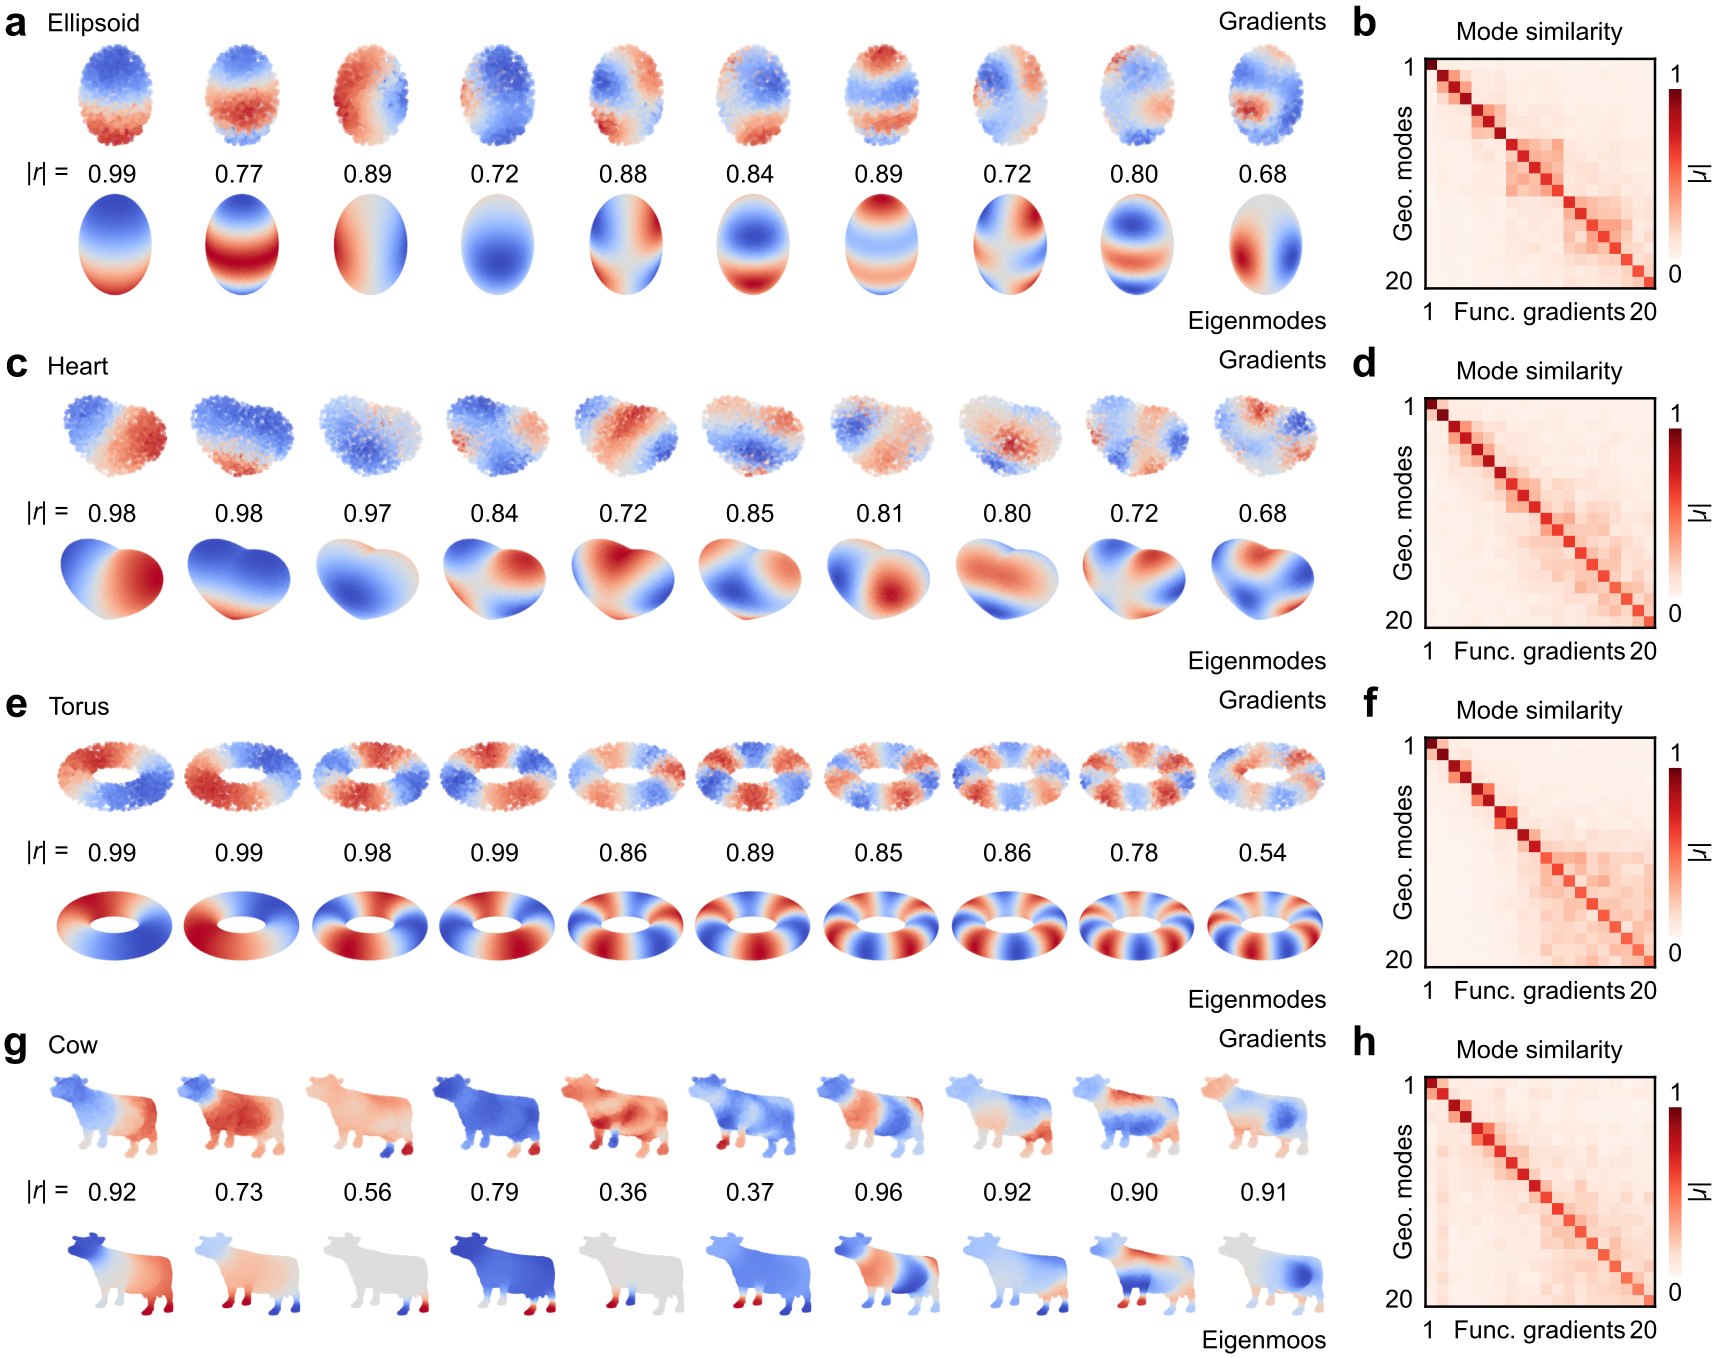
\includegraphics[width=1.0\linewidth]{figures/supp_geometries.pdf}
    \caption{Comparison of functional connectivity gradients and geometric eigenmodes in various geometries. (\textbf{a}) Gradients and eigenmodes of an ellipsoid shape; absolute correlations $|r|$ are indicated for the first 10 mode pairs (one representative simulation). (\textbf{b}) Eigenmode-gradient correlation matrix for the ellipsoid geometry, averaged across 10 coordinate sets. (\textbf{c}) Gradients and eigenmodes of a heart shape. (\textbf{d}) Eigenmode-gradient correlation matrix for the heart geometry, averaged across 10 coordinate sets. (\textbf{e}) Gradients and eigenmodes of a torus shape. (\textbf{f}) Eigenmode-gradient correlation matrix for the torus geometry, averaged across 10 coordinate sets. (\textbf{g}) Gradients and eigenmodes of a cow shape. (\textbf{h}) Eigenmode-gradient correlation matrix for the cow geometry, averaged across 10 coordinate sets.}
    \label{supp_geometries}
\end{figure*}

\newpage

\begin{figure*}[t]
    \centering
    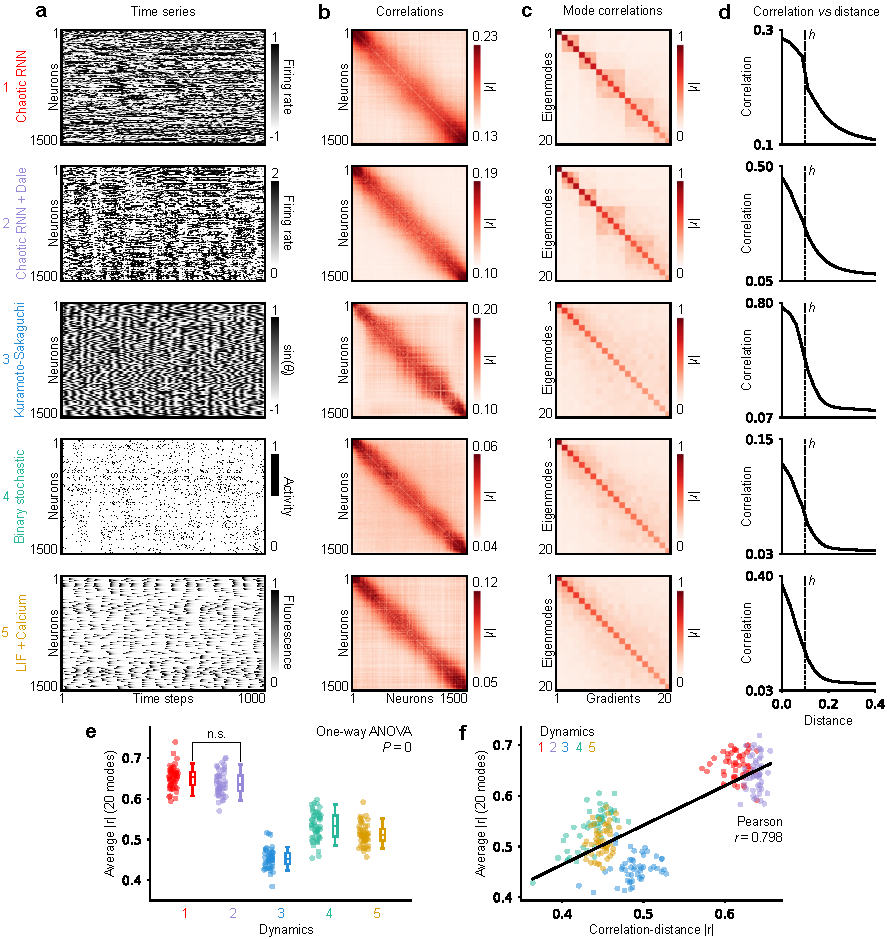
\includegraphics[width=1.0\linewidth]{figures/supp_dynamics.pdf}
    \caption{Eigenmode-gradient correlations in ellipsoid for different dynamical systems. (\textbf{a}) Example simulated time series from five dynamical models, indicated on the left and detailed in Methods; all simulations are embedded in the ellipsoid geometry. (\textbf{b}) Example pairwise neuronal activity correlations for each model, averaged across 100 simulations; the matrix is sorted to follow the $z$ axis of the ellipsoid. (\textbf{c}) Eigenmode-gradient correlation matrices for each dynamical model, averaged across 10 ellipsoids. (\textbf{d}) Average correlation-distance relationships for each dynamical model; a dashed line indicates the connectivity radius $h$ of neurons. (\textbf{e}) Average eigenmode-gradient correlations for each dynamical model (50 different simulations, averaged over mode pairs); different models yield statistically different eigenmode-gradient correlations (one-way ANOVA, $P=0$). (\textbf{f}) Eigenmode-gradient $|r|$ as a function of the correlation-distance $|r|$ for the five different models; dynamical models whose correlations are more tightly coupled to euclidean distance yield a better correspondence (Pearson $r=0.798$), which suggests that dynamics with many spurious or long-range correlations degrade the geometric gradients. }
    \label{supp_dynamics}
\end{figure*}

\newpage

\begin{figure*}[t]
    \centering
    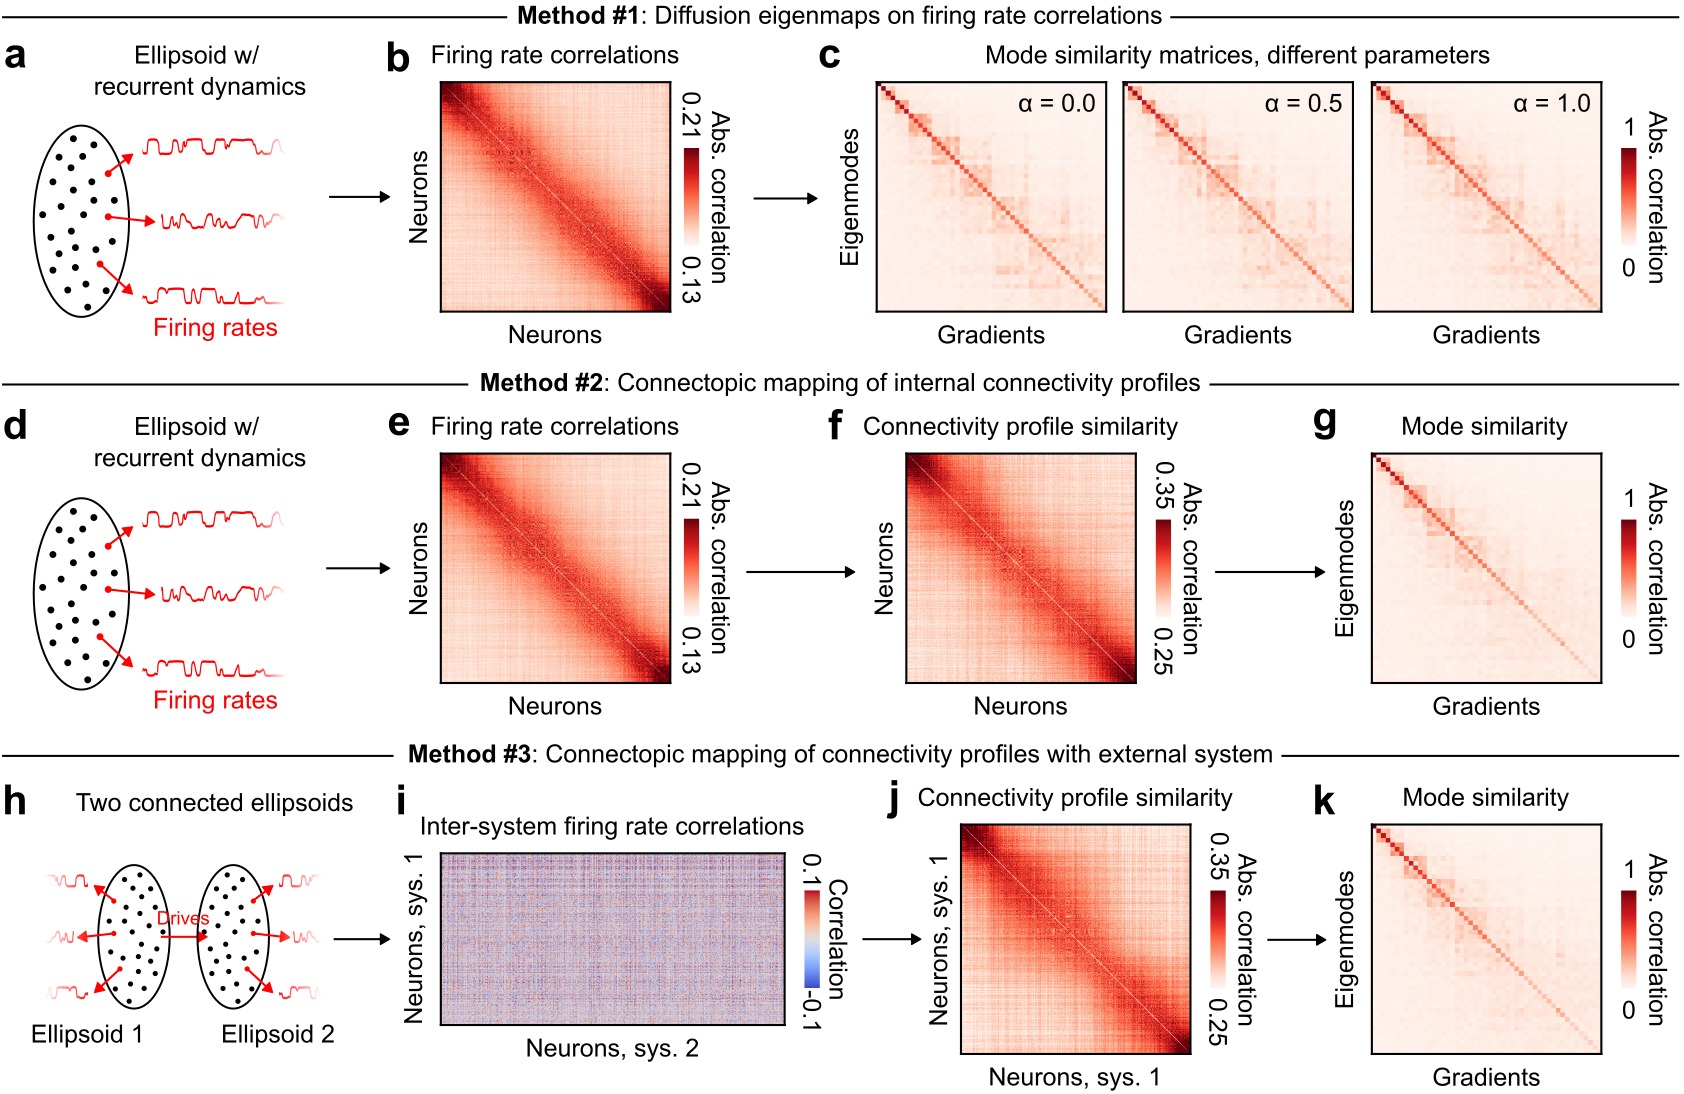
\includegraphics[width=1.0\linewidth]{figures/supp_gradient_methods.pdf}
    \caption{Derivation of geometric gradients using various gradient analysis methods. (\textbf{a}-\textbf{c}) Method 1 uses the diffusion maps algorithm on the firing rate correlation matrix to compute gradients, yielding results that are mostly independent of the $\alpha$ parameter controlling the effect of local density on the diffusion process. (\textbf{d}-\textbf{g}) Method 2 adds one extra step to the first method by computing the connectivity profile similarity from the correlation matrix before computing gradients. (\textbf{h}-\textbf{i}) Method 3 approximates the connectopic mapping procedure used in Pang et al\cite{pang2023geometric}, who derived subcortical gradients from their temporal association with cortical activity. Here, two interconnected systems are simulated, one smaller representing a subcortical region, and one larger representing external regions like the cortex. Time series from both ellipsoids are correlated to each other, and then the connectivity profile similarity matrix is used to compute gradients. Overall, this supplementary analysis demonstrates that geometric gradients can be obtained from gradient derivation methods that vary in their sequence of numerical operations, highlighting their methodological robustness.}
    \label{supp_methods}
\end{figure*}

\newpage

\begin{figure*}[t]
    \centering
    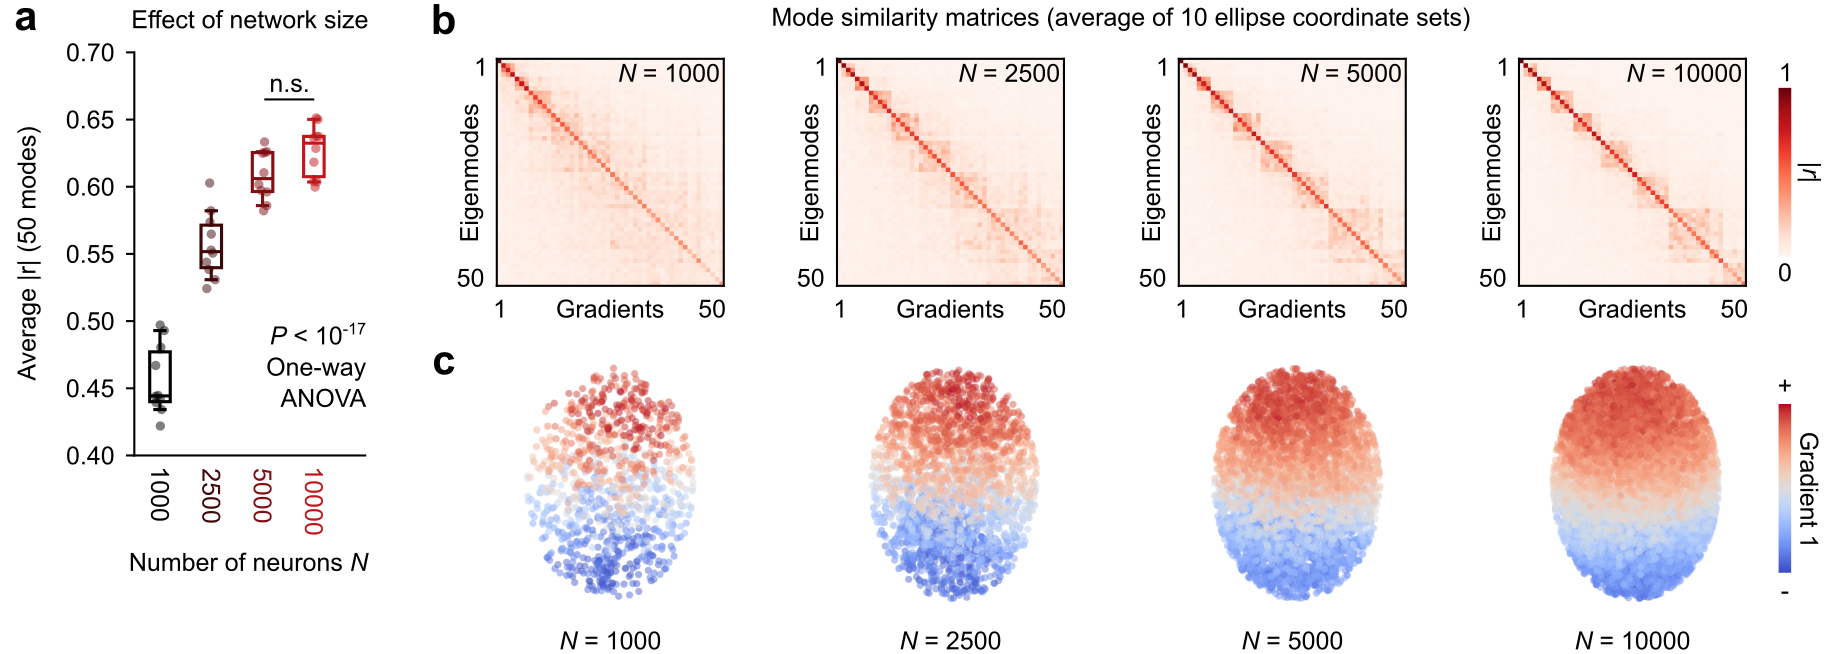
\includegraphics[width=1.0\linewidth]{figures/supp_network_size.pdf}
    \caption{Eigenmode-gradient correlations in ellipsoid for different network sizes. (\textbf{a}) Average eigenmode-gradient correlation (averaged over 50 mode pairs) for four different network sizes; denser networks exhibit gradients that correlate more with geometric eigenmodes (one-way ANOVA, $P<10^{-17}$). (\textbf{b}) Eigenmode-gradient correlation matrices for different network sizes (indicated in the top right matrix corners), averaged over 10 ellipsoids. (\textbf{c}) Neuron centroids colored by the numerical values of the first functional gradient for increasing network sizes.}
    \label{supp_network_size}
\end{figure*}

\newpage

\begin{figure*}[t]
    \centering
    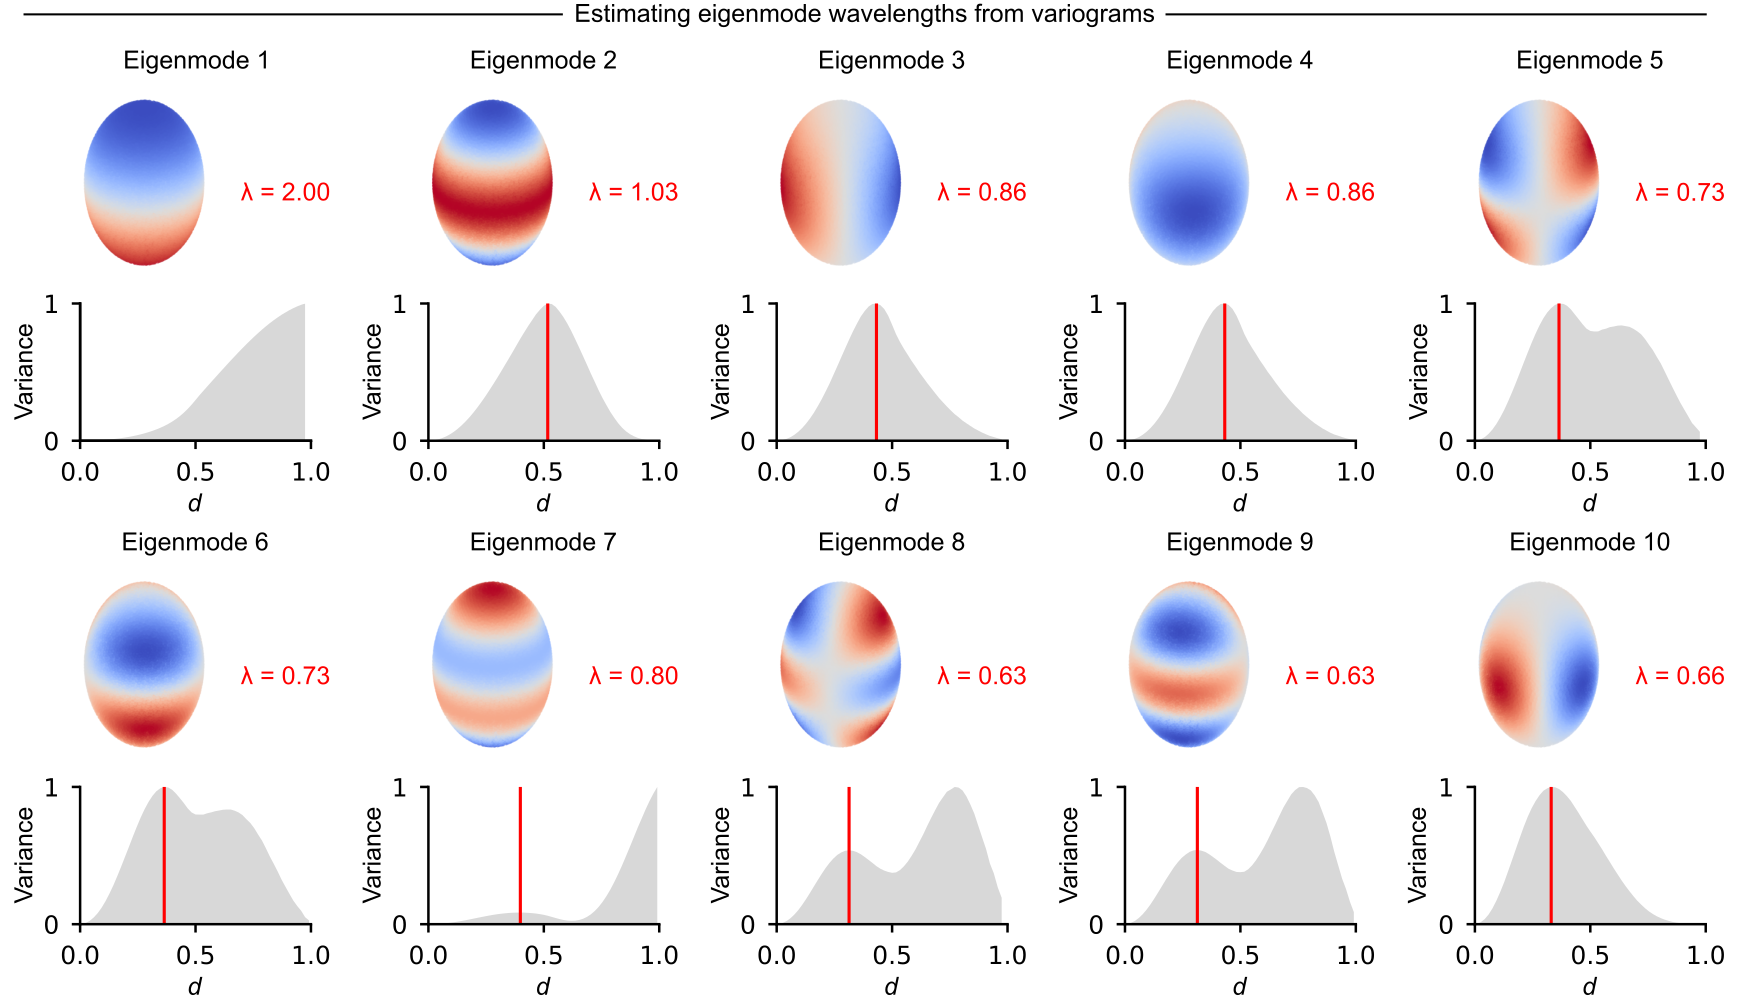
\includegraphics[width=1.0\linewidth]{figures/supp_variograms.pdf}
    \caption{Estimating eigenmode wavelengths using their spatial variograms. The first 10 ellipsoid eigenmodes are plotted alongside their wavelengths (top rows), which are estimated from the first peak of each variogram (bottom rows, Methods).}
    \label{supp_variograms}
\end{figure*}

\newpage

\begin{figure*}[t]
    \centering
    \includegraphics[width=1.0\linewidth]{figures/supp_lineprofiles.pdf}
    \caption{Individual gradient-eigenmode correlation curves for varying network parameters. (\textbf{a}) Normalized row profiles of the matrix in \ref{fig3}\textbf{b}, corresponding to individual eigenmode-gradient correlation curves at varying connectivity radii $h$. (\textbf{b}) Normalized row profiles of the matrix in Fig. \ref{fig3}\textbf{e}, corresponding to individual eigenmode-gradient correlation curves at varying fractions of edges swapped $\rho_{\text{swaps}}$. (\textbf{c}) Normalized row profiles from the two previous panels, horizontally aligned and centered at $|r|=0.5$, highlighting the very different effects of either increasing the connectivity radius $h$ (in red, abrupt decay) or randomly swapping edges (in blue, linear decay).}
    \label{supp_lineprofiles}
\end{figure*}

\newpage

\begin{figure*}[t]
    \centering
    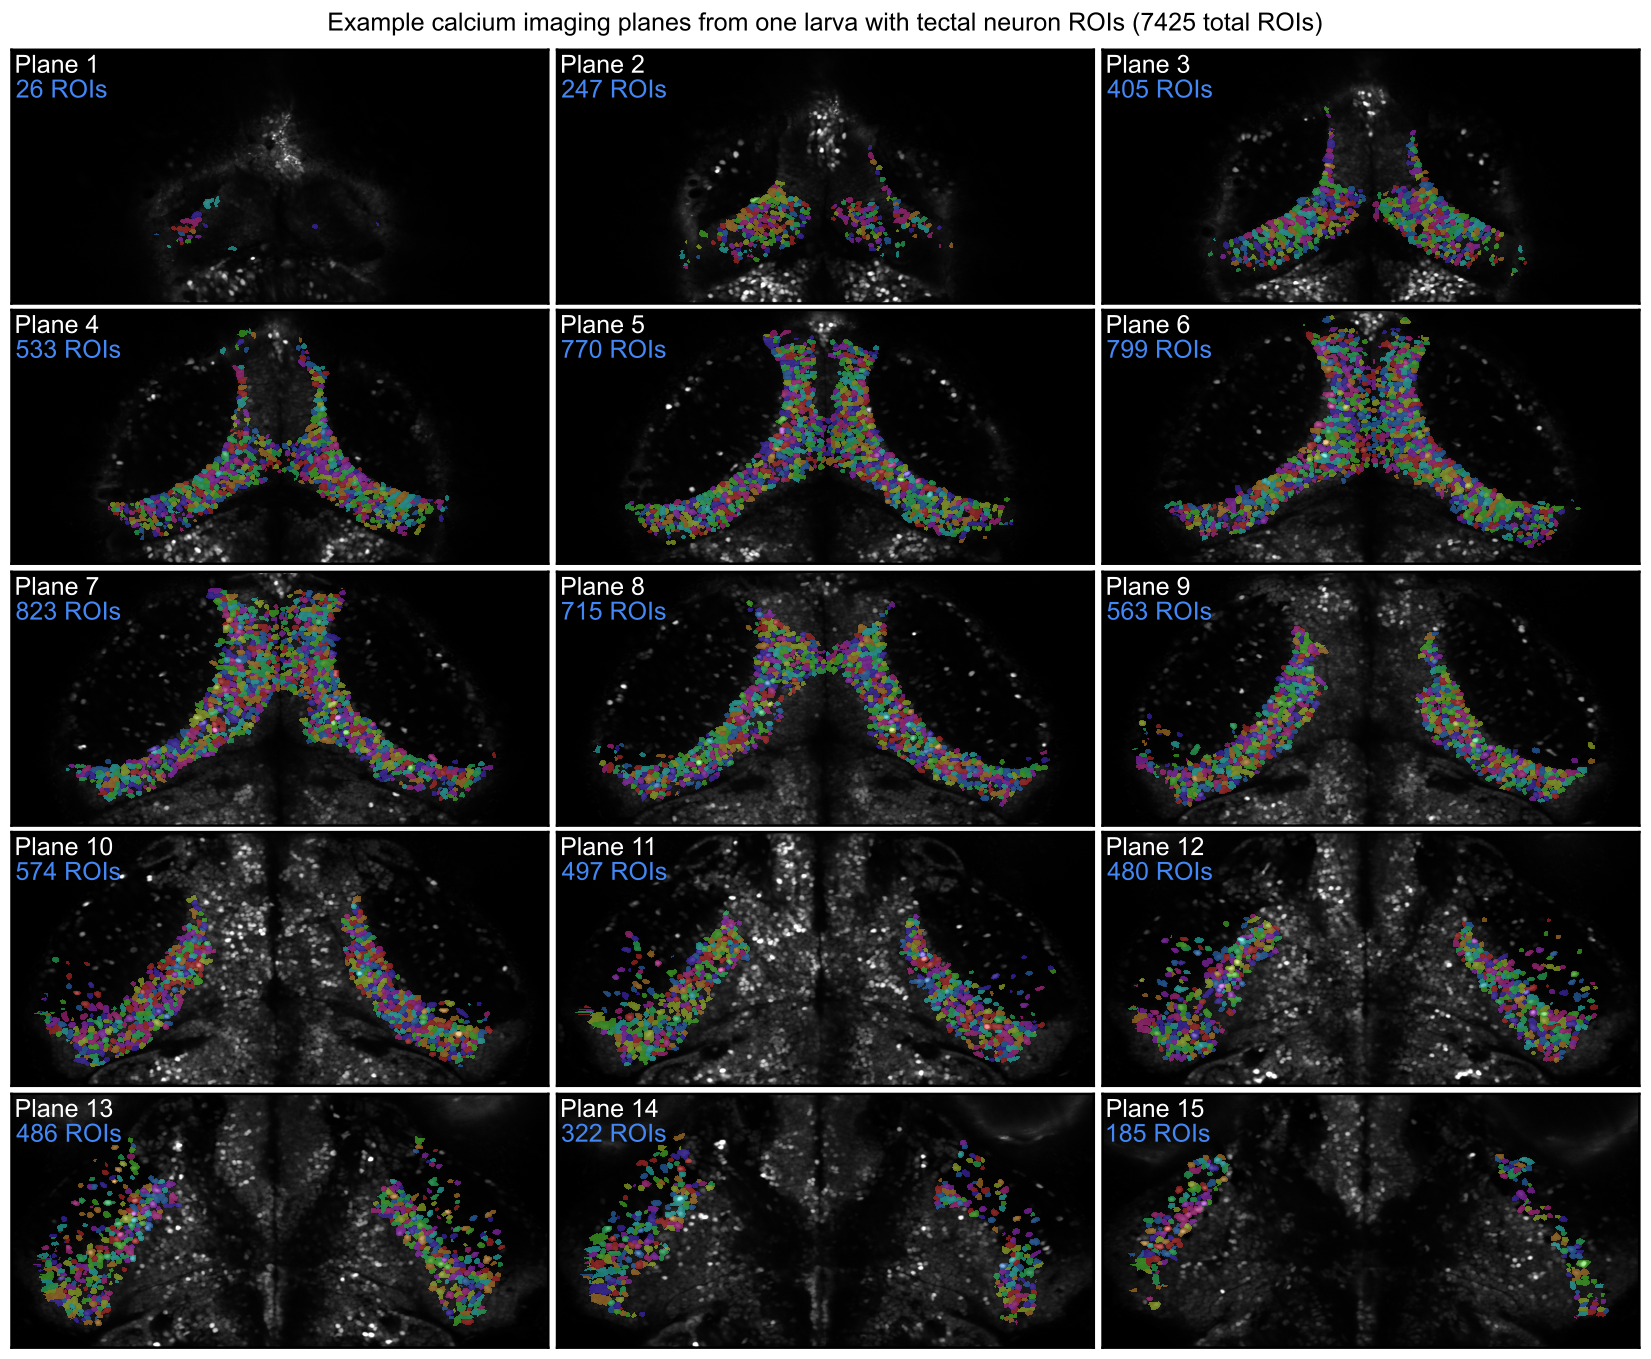
\includegraphics[width=1.0\linewidth]{figures/supp_imagingplanes.pdf}
    \caption{Temporal averages of two-photon calcium imaging planes from one example animal, with pseudocolored nuclei located within the optic tectum identified using Cellpose 2.0. The number of detected regions of interest (ROIs) is indicated on each plane. Imaging volumes extend from the most dorsal (top left) to the most ventral (bottom right) parts of the tectum across both hemispheres to ensure that the entire 3D structure is properly sampled.}
    \label{supp_imagingplanes}
\end{figure*}

\newpage

\begin{figure*}[t]
    \centering
    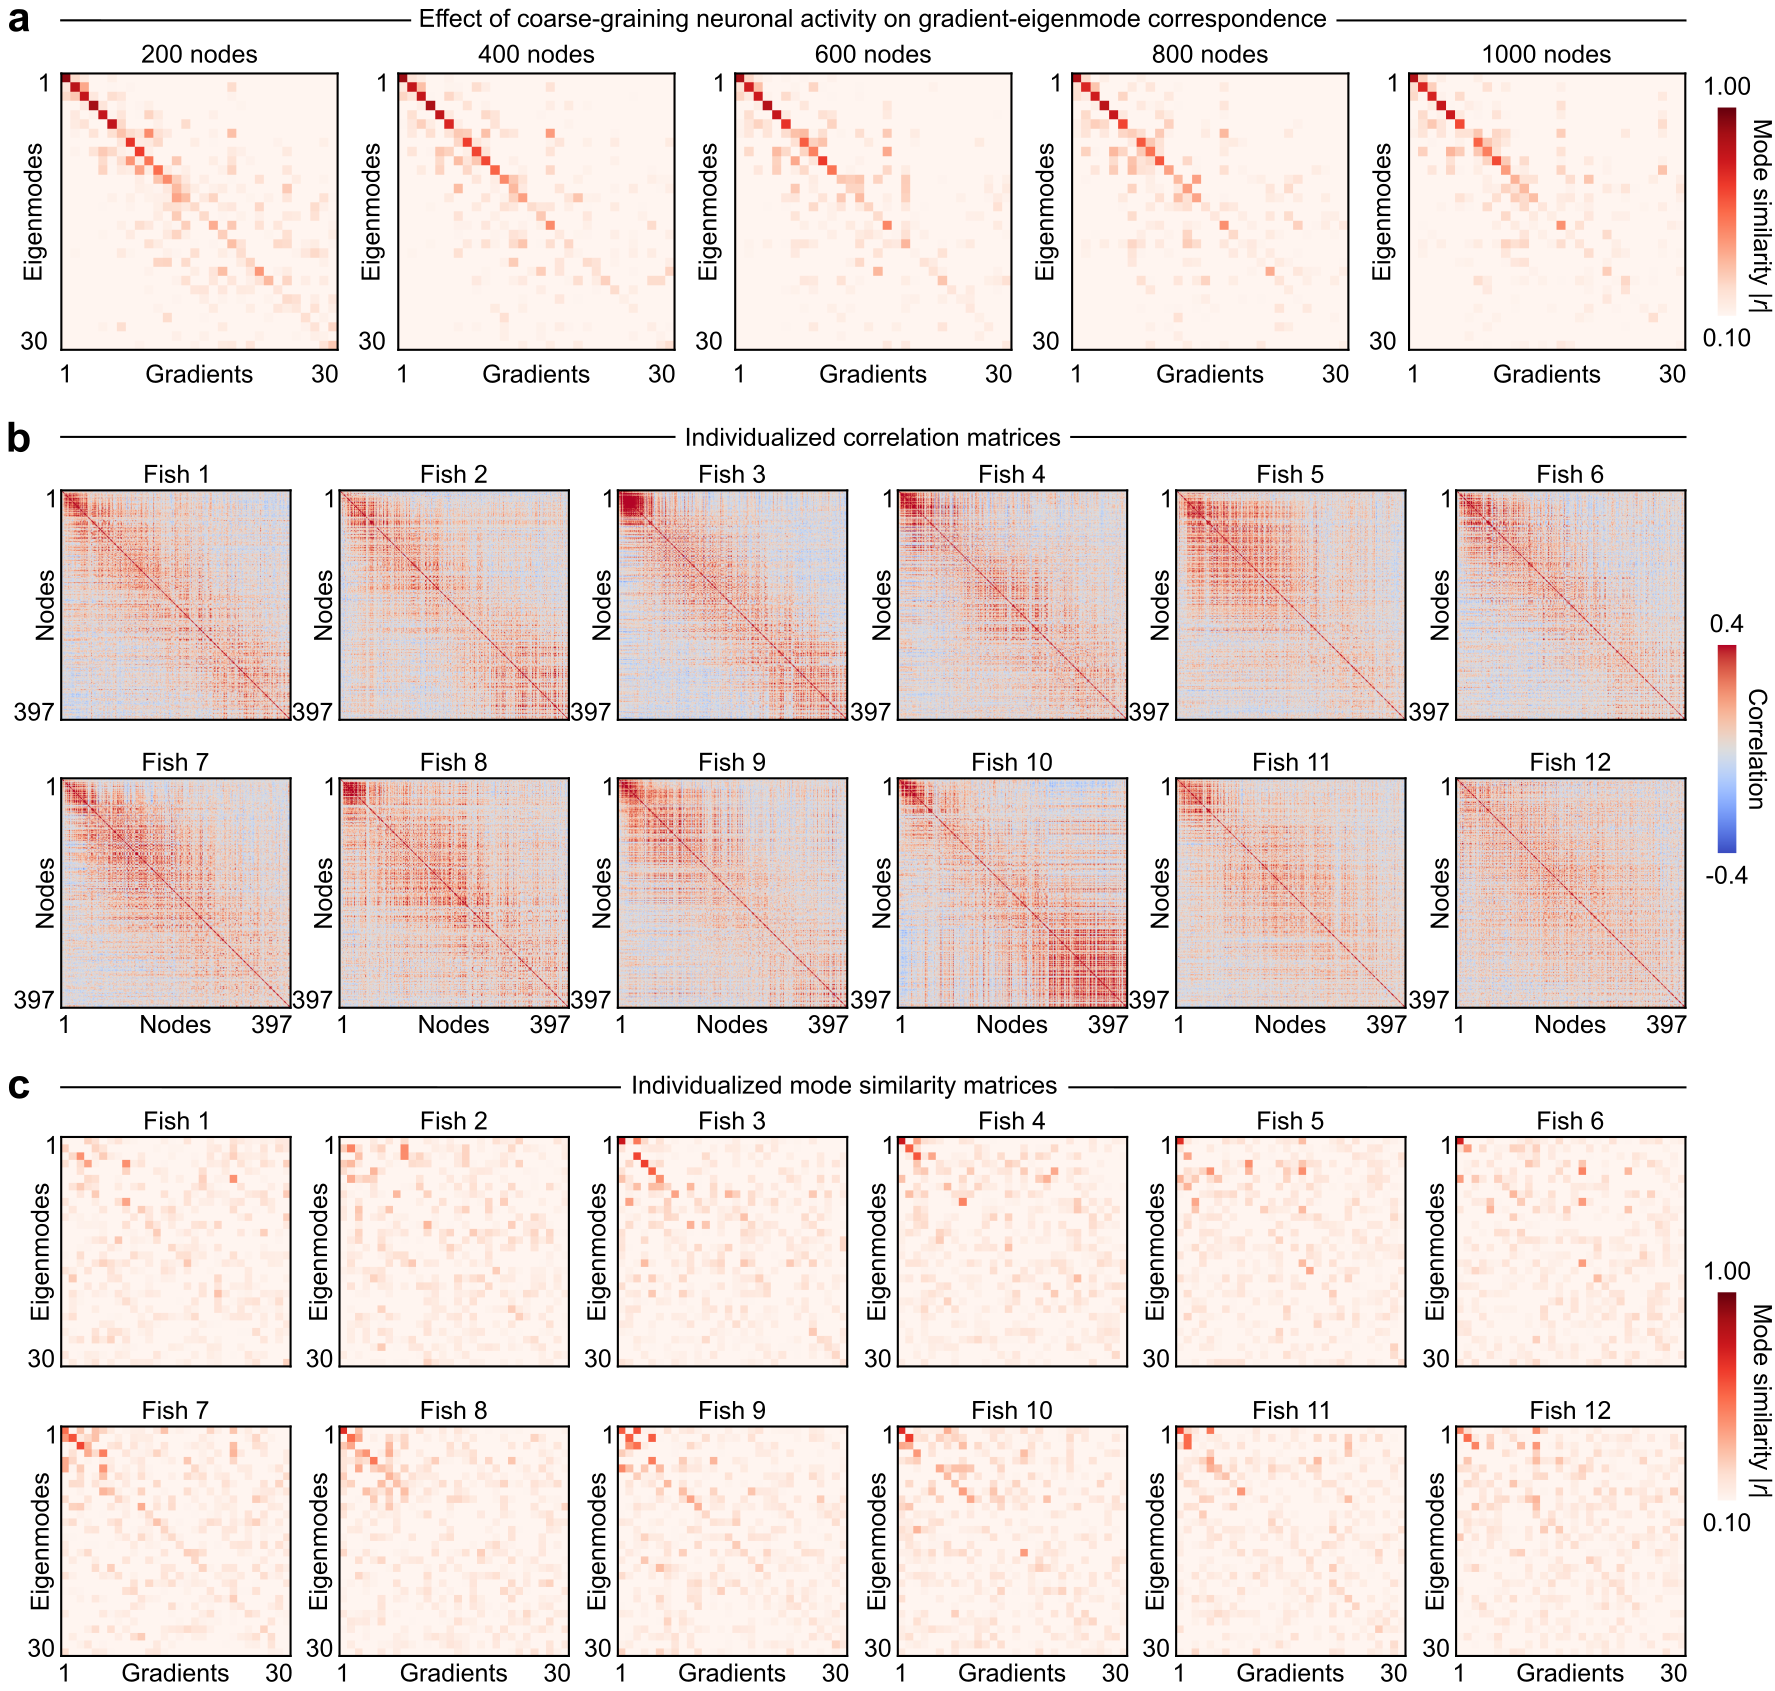
\includegraphics[width=1.0\linewidth]{figures/supp_coarsegraining.pdf}
    \caption{Effect of coarse-graining and averaging on geometric gradients. (\textbf{a}) Eigenmode-gradient correlation matrices for varying numbers of network nodes in the optic tectum; notice the minimal effect of spatial resolution on the eigenmode-gradient correlations. (\textbf{b}) Correlation matrices of optic tectum node activity for 12 different larvae, sorted from anterior to posterior nodes. (\textbf{c}) Eigenmode-gradient correlation matrices calculated on the individual correlation matrices from the previous panel; notice the poor quality of the correspondence in most animals. This suggests that individual imaging sessions insufficiently sample the correlation structure of the optic tectum.}
    \label{supp_coarsegraining}
\end{figure*}

\newpage

\begin{figure*}[t]
    \centering
    \includegraphics[width=1.0\linewidth]{figures/supp_noise.pdf}
    \caption{Influence of experimental noise on the geometric cutoff wavelength. (\textbf{a}) Five example single-neuron fluorescence time series, with varying noise levels; black, raw traces; red, raw traces with numerical noise drawn from a normal distribution with 3 times the standard deviation of the data. (\textbf{b}) Absolute correlation $|r|$ averaged across 30 eigenmode-gradient pairs for varying noise levels applied to fluorescence time series; red, average curve; black dots, 10 replicates per noise level. (\textbf{c}) Cutoff wavelength inferred from a piecewise linear fit on eigenmode-gradient correlation matrix diagonals for varying noise levels; red, average curve; black dots, 10 replicates per noise level; despite a gradual decrease of correlations observed in $\textbf{b}$, no significant cutoff wavelength differences are observed until noise levels reach $3.5\sigma_{\text{data}}$ (One-way ANOVA, $P=0.105$, $F=1.929$). This analysis suggests that experimental noise has a negligible influence on the position of the cutoff point in the eigenmode-gradient mapping.}
    \label{supp_noise}
\end{figure*}

\newpage

\begin{figure*}[t]
    \centering
    \includegraphics[width=1.0\linewidth]{figures/supp_tectum_cutoff.pdf}
    \caption{Two different methods can retrieve the connectivity radius $h$ of the optic tectum based on numerical simulations. (\textbf{a}) Method 1 identifies cutoff points at the level of individual eigenmodes by varying the connectivity radius $h$ over many simulations, which generates curves with abrupt drop-offs for each eigenmode; this approach is used in Fig. \ref{fig3}. (\textbf{b}) The $h$ cutoff points identified for each eigenmode using method 1 are linearly correlated to eigenmode spatial wavelengths (averaged over 10 coordinate sets, 100 simulations per set); CI, confidence interval. (\textbf{c}) In contrast, method 2 identifies cutoff points at the mode ensemble level, rather than per individual eigenmode. This is achieved by fitting a piecewise linear relationship to the eigenmode-gradient correlation matrix diagonal, with the elbow of the curve corresponding to the cutoff point. (\textbf{d}) Cutoff points identified using this method are also linearly correlated with the connectivity radius $h$ used in simulations (averaged over 10 coordinate sets, 100 simulations per set). While method 1 can only be applied to numerical simulations, method 2 is applicable to real data, as it requires a single eigenmode-gradient correlation matrix to estimate the $h$ parameter, provided a linear relationship has been established from numerical simulations beforehand. This approach is used in Fig. \ref{fig7} to estimate the arbor size of tectal neurons.}
    \label{supp_tectum_cutoff}
\end{figure*}

\newpage

\begin{figure*}[t]
    \centering
    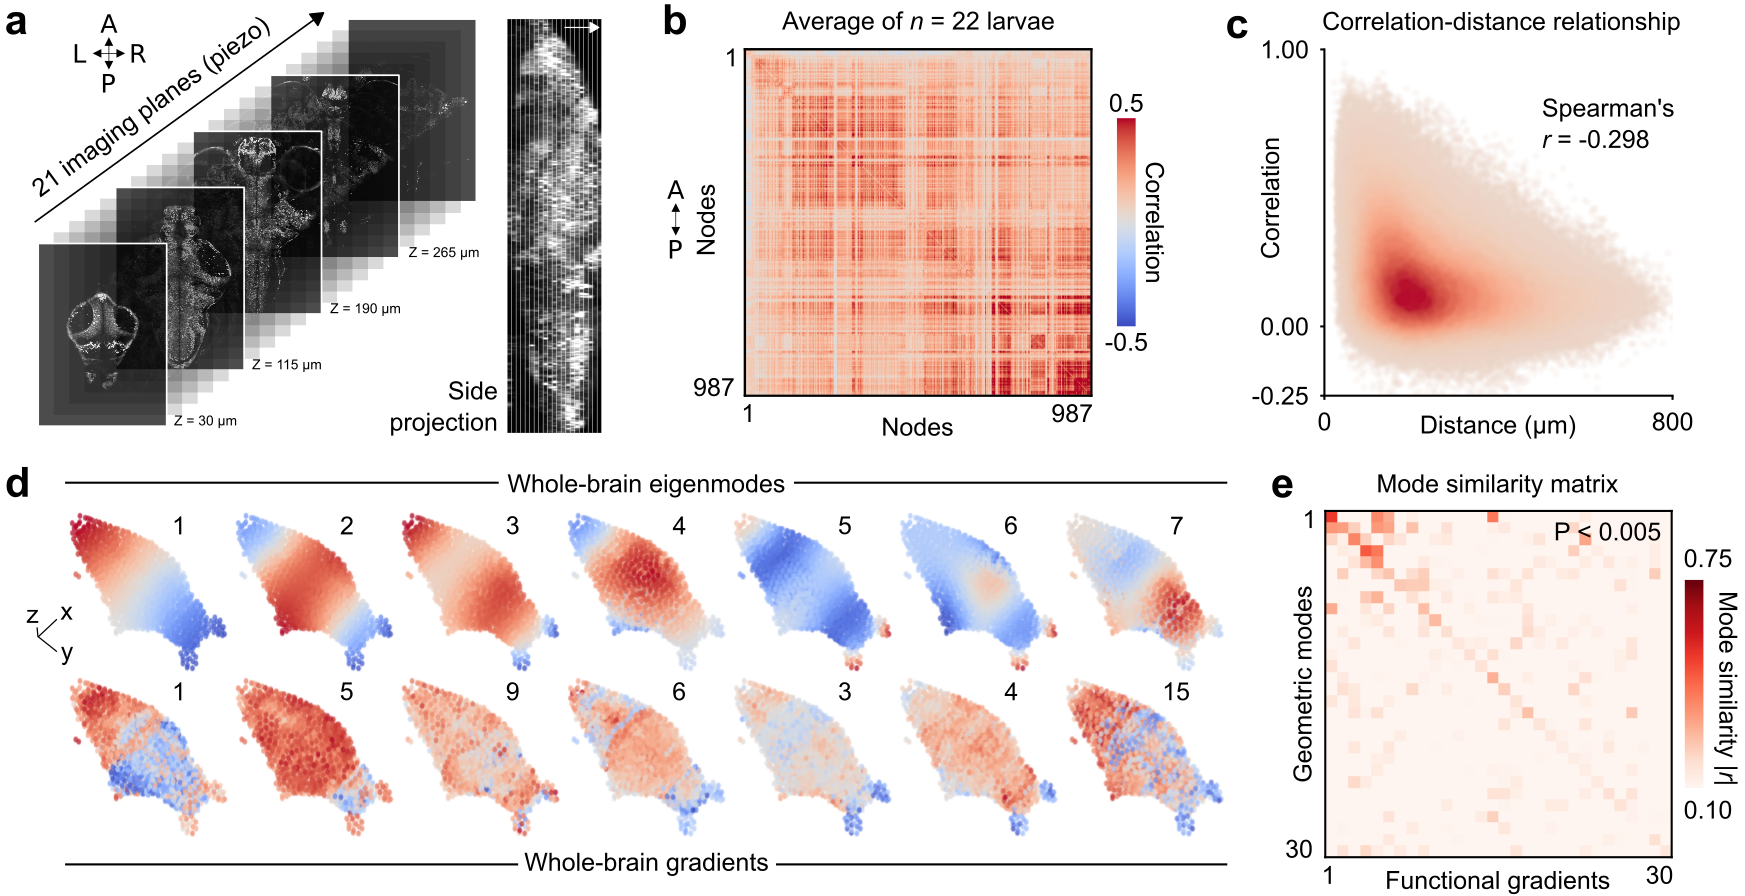
\includegraphics[width=1.0\linewidth]{figures/supp_wholebrain.pdf}
    \caption{Whole-brain functional connectivity gradients do not reflect geometric eigenmodes. (\textbf{a}) Whole-brain imaging using two-photon microscopy; the dataset and imaging parameters are detailed in a previous study\cite{legare2025structural}. (\textbf{b}) Group-averaged whole-brain functional connectivity ($n=22$ larvae, 5-7 days post-fertilization, 10 minutes of spontaneous activity); neurons are mapped in 987 nodes per hemisphere, and correlations are averaged across hemispheres. (\textbf{c}) Correlation-distance relationship of whole-brain FC (Spearman's $r=-0.298$). (\textbf{d}) Top, whole-brain geometric eigenmodes; bottom, whole-brain functional connectivity gradients; both mode ensembles are projected onto 987 nodes per brain hemisphere and colors are scaled arbitrarily. (\textbf{e}) Whole-brain eigenmode-gradient correlation matrix; the correspondence is significant at the group level, that is, when eigenmode-gradient correlations are averaged over the matrix diagonal ($P<0.005$, 1000 SA-preserving spatial permutations). Nevertheless, the eigenmode-gradient correspondence is substantially worse at the whole-brain level than within the optic tectum.}
    \label{supp_wholebrain}
\end{figure*}

\newpage

\begin{figure*}[t]
    \centering
    \includegraphics[width=1.0\linewidth]{figures/supp_smoothing.pdf}
    \caption{Spatial filtering drives geometric eigenmodes in both optic tectum and whole-brain calcium imaging data. (\textbf{a}) Tectal (top) and whole-brain (bottom) FC matrices for varying spatial filtering kernel sizes, indicated on each matrix ($n=12$ larvae for tectal data, $n=22$ larvae for whole-brain data). (\textbf{b}) Eigenmode-gradient correlation $|r|$ averaged over 30 mode pairs for the optic tectum (red) and the entire brain (black) at varying filtering kernel sizes; optima are indicated for each curve. While numerical simulations in Fig. \ref{fig5} demonstrate potentially nonlinear effects, spatial filtering applied to real data monotonously increases the correlation between eigenmodes and gradients before an optimum is reached. (\textbf{c}) Predicted connectivity radii inferred using the piecewise linear fit method on the mode correlation matrix diagonal at varying filtering levels (optic tectum only). Spatial filtering does not change the predicted connectivity radius, as radii at varying filtering kernels mostly contained within the 95\% confidence interval of the predicted radius at $\sigma=0$ $\mu$m; the confidence interval arises from the linear regression in Supp. Fig. \ref{supp_tectum_cutoff}\textbf{d}.}
    \label{supp_smoothing}
\end{figure*}

\newpage
\clearpage

\section*{Supplementary Mathematical Note}

\subsection*{Calculation of filtering-induced correlations}

We demonstrate the claim made in the main text that the expected correlations induced by filtering uncorrelated gaussian noise signals are given by
\begin{align*}
    \Tilde{c}_{ij} \approx e^{-d_{ij}^2/4\sigma^2}.
\end{align*}
Let us begin with the Pearson correlation coefficient
\begin{align*}
    c_{ij} & = \frac{\expval{f_if_j}-\expval{f_i}\expval{f_j}}{\sigma_{f_i}\sigma_{f_j}},
    %\label{eq:exp_coefficient}
\end{align*}
where $f_i$ is the random variable corresponding to the signal measured from node $i$, $\expval{f_i}$ is its expected value, and $\sigma_{f_i}$ is its standard deviation.
Without loss of generality, we assume that $\expval{f_i} = 0$ for all $i$, which implies that
\begin{align}
    c_{ij} & = \frac{\expval{f_if_j}}{\sigma_{f_i}\sigma_{f_j}} .
    \label{eq:centered-correlation}
\end{align}
%on an observed unknown network, for instance. If we treat those signals as independent and with mean $0$, the expected coefficient is simply
% \begin{align*}
%     c_{ij} &= \frac{\expval{f_i}\expval{f_j}-\expval{f_i}\expval{f_j}}{\sigma_{f_i}\sigma_{f_j}} = 0.
% \end{align*}
% Now, we introduce spatial filtering to the signal. This procedure consists of convoluting the signal with a gaussian filter, which yields
The spatial filtering considered in the main text consists in the convolution of the activities with a Gaussian filter, meaning that the signal measured from node $i$ becomes
\begin{align*}
    \Tilde{f}_i &= \frac{1}{\sqrt{2\pi}\sigma N}\sum_{k=1}^N e^{-\nicefrac{d_{ik}^2}{2\sigma^2}}f_k,
\end{align*}
where $\sigma$ is the standard deviation of the Gaussian filter, $N$ is the number of nodes in the network, and $d_{ik}$ is the distance between nodes $i$ and $k$.
%all $f_k$ have mean $0$, the filtered signals $\Tilde{f}_i$ also have mean $0$.
The covariance between these filtered signals is
\begin{align*}
    \expval{\Tilde{f}_i\Tilde{f}_j} - \expval{\Tilde{f}_i}\expval{\Tilde{f}_j}
    & = \frac{1}{2\pi\sigma^2N^2}\expval{\qty(\sum_{k=1}^N e^{-\nicefrac{d_{ik}^2}{2\sigma^2}}f_k)\qty(\sum_{\ell=1}^N e^{-\nicefrac{d_{j\ell}^2}{2\sigma^2}}f_\ell)}
      - \frac{1}{2\pi\sigma^2N^2}\expval{\sum_{k=1}^N e^{-\nicefrac{d_{ik}^2}{2\sigma^2}}f_k} \expval{\sum_{\ell=1}^N e^{-\nicefrac{d_{j\ell}^2}{2\sigma^2}}f_\ell} \\
    & = \frac{1}{2\pi\sigma^2N^2}\sum_{k, \ell =1}^N e^{\nicefrac{-(d_{ik}^2+d_{j\ell}^2)}{2\sigma^2}}\expval{f_kf_\ell}
      - \frac{1}{2\pi\sigma^2N^2}\qty(\sum_{k=1}^N e^{-\nicefrac{d_{ik}^2}{2\sigma^2}}\expval{f_k}) \qty(\sum_{\ell=1}^N e^{-\nicefrac{d_{j\ell}^2}{2\sigma^2}}\expval{f_\ell}) \\
    & = \frac{1}{2\pi\sigma^2N^2}\sum_{k, \ell =1}^N e^{\nicefrac{-(d_{ik}^2+d_{j\ell}^2)}{2\sigma^2}}\qty(\expval{f_kf_\ell} - \expval{f_k}\expval{f_\ell}) \\
    & = \frac{1}{2\pi\sigma^2N^2}\sum_{k, \ell =1}^N e^{\nicefrac{-(d_{ik}^2+d_{j\ell}^2)}{2\sigma^2}}\expval{f_kf_\ell} \\
    & = \frac{1}{2\pi\sigma^2N^2}\sum_{k, \ell =1}^N e^{\nicefrac{-(d_{ik}^2+d_{j\ell}^2)}{2\sigma^2}}\sigma_{f_k}\sigma_{f_\ell} c_{k\ell} ,
\end{align*}
where we used the fact that $\expval{f_i} = 0$ for all $i$, and invoked Eq.~\eqref{eq:centered-correlation}.
The variance of each filtered signal simplifies to
\begin{align*}
    \sigma^2_{\Tilde{f}_i}
      = \expval{\Tilde{f}_i^2} - \expval{\Tilde{f}_i}^2
      = \frac{1}{2\pi\sigma^2N^2}\sum_{k, \ell =1}^N e^{\nicefrac{-d_{ik}^2}{\sigma^2}}\expval{f_kf_\ell}
      = \frac{1}{2\pi\sigma^2N^2}\sum_{k, \ell =1}^N e^{\nicefrac{-d_{ik}^2}{\sigma^2}}\sigma_{f_k}\sigma_{f_\ell} c_{k\ell} .
\end{align*}
The correlation between the filtered signals therefore is
\begin{align*}
  \Tilde{c}_{ij}
    & = \frac{\expval{\Tilde{f}_i\Tilde{f}_j} - \expval{\Tilde{f}_i}\expval{\Tilde{f}_j}}{\sigma_{\Tilde{f}_i} \sigma_{\Tilde{f}_j}} \\
    & = \frac{\sum_{k, \ell =1}^N e^{\nicefrac{-(d_{ik}^2+d_{j\ell}^2)}{2\sigma^2}}\sigma_{f_k}\sigma_{f_\ell} c_{k\ell}}%
      {\sqrt{\qty(\sum_{k, \ell =1}^N e^{\nicefrac{-d_{ik}^2}{\sigma^2}}\sigma_{f_k}\sigma_{f_\ell} c_{k\ell}) \qty(\sum_{k, \ell =1}^N e^{\nicefrac{-d_{jk}^2}{\sigma^2}}\sigma_{f_k}\sigma_{f_\ell} c_{k\ell})}} .
\end{align*}

We now assume that the raw signals are independently and identically distributed, which further implies that $\expval{f_kf_\ell} = \expval{f_k^2}\delta_{k\ell} \equiv \sigma_{f}^2\delta_{k\ell}$ and that $c_{k\ell} = \delta_{k\ell}$, where $\delta_{k\ell}$ is the Kroenecker delta.
The correlation between the filtered signals simplifies to
% Since the raw signals are independent, $\expval{f_kf_\ell} = \expval{f_k^2}\delta_{k\ell} = \sigma_{f_k}^2\delta_{k\ell}$, with $\delta_{k\ell}$ the Kronecker delta. The covariance is therefore
% \begin{align*}
%     \expval{\Tilde{f}_i\Tilde{f}_j} &= \frac{1}{2\pi\sigma^2N^2}\sum_{k = 1}^N e^{\nicefrac{-(d_{ik}^2+d_{jk}^2)}{2\sigma^2}}\sigma_{f_k}^2.
% \end{align*}
% For the standard deviations,
% \begin{align*}
%     \sigma^2_{\Tilde{f}_i} &= \expval{\Tilde{f}_i^2}\\
%     &= \frac{1}{2\pi\sigma^2N^2}\expval{\qty(\sum_{k=1}^N e^{-\nicefrac{d_{ik}^2}{2\sigma^2}}f_k)\qty(\sum_{\ell=1}^N e^{-\nicefrac{d_{i\ell}^2}{2\sigma^2}}f_\ell)}\\
%     &= \frac{1}{2\pi\sigma^2N^2}\expval{\sum_{k, \ell =1}^N e^{-(\nicefrac{d_{ik}^2 + d_{i\ell}^2)}{2\sigma^2}}f_kf_\ell}\\
%     &= \frac{1}{2\pi\sigma^2N^2}\sum_{k=1}^N e^{-\nicefrac{d_{ik}^2}{\sigma^2}}\sigma_{f_k}^2.
% \end{align*}
% If all the signals are i.i.d, that is they all have the same variance, then the expected correlation between the filtered signals is
\begin{align}
    \Tilde{c}_{ij} &= \frac{\sum_{k = 1}^N e^{\nicefrac{-(d_{ik}^2+d_{jk}^2)}{2\sigma^2}}}{\sqrt{\qty(\sum_{k=1}^N e^{-\nicefrac{d_{ik}^2}{\sigma^2}})\qty(\sum_{\ell=1}^N e^{-\nicefrac{d_{j\ell}^2}{\sigma^2}})}} > 0 ,
    \label{eq:indiced-correlation}
\end{align}
which demonstrates that filtering uncorrelated induces correlations indeed.

Exact computation of $\Tilde{c}_{ij}$ depends on the distribution of the distances between the nodes and on the precise geometry of the manifold, and cannot be further carried out analytically in general.
However, assuming that nodes are distributed uniformly in the manifold, and ignoring the effect of the manifold's boundaries, we can use a continuous approximation which becomes exact as $N\to \infty$.
Under these assumptions, both sums in the denominator can be approximated as
\begin{align*}
    \sum_{k=1}^N e^{-\nicefrac{d_{ik}^2}{\sigma^2}}
      \approx \int_0^{2\pi}\int_0^\infty e^{-r^2/\sigma^2}r\dd r\dd\theta
      = \pi \sigma^2 ,
\end{align*}
which is independent of $i$.
The denominator in Eq.~\eqref{eq:indiced-correlation} can therefore be approximated by $\pi\sigma^2$. 

We can approximate the numerator in Eq.~\eqref{eq:indiced-correlation} with a similar approach, combined with the law of cosines and with the following geometric construction:
%
\begin{center}
\begin{tikzpicture}

    % Define the center, the point on the circle, and the external point
    \coordinate (i) at (0,0); % Center of the circle
    \coordinate (k) at (1,2); % Point on the circle
    \coordinate (j) at (4,0); % Point outside the circle

    % Draw the circle
    \draw (i) circle[radius=sqrt(5)];

    % Draw the radius
    \draw[dashed] (i) -- (k);

    % Draw the lines from j to i and j to k
    \draw[dashed] (j) -- (i);
    \draw[dashed] (j) -- (k);

    % Draw the center, boundary point, and external point
    \fill (i) circle[radius=2pt];
    \fill (k) circle[radius=2pt];
    \fill (j) circle[radius=2pt];

    % Label the center, boundary point, and external point
    \node at (i) [label=left:$i$] {};
    \node at (k) [label=above:$k$] {};
    \node at (j) [label=above:$j$] {};

    % Label the radius
    \node at ($(i)!0.5!(k)$) [above left] {$r$};

    % Label the lines
    \node at ($(i)!0.4!(j)$) [below right] {$d_{ij}$};
    \node at ($(k)!0.5!(j)$) [above right] {$d_{jk}$};
    \pic [draw, ->, "$\theta$", angle eccentricity=1.5] {angle = j--i--k};
\end{tikzpicture}
\end{center}

With the law of cosines, 
\begin{equation*}
    d_{jk}^2 = r^2+d_{ij}^2-2rd_{ij}\cos\theta.
\end{equation*}
As such, the integral approximating the numerator is
\begin{align*}
    \sum_{k = 1}^N e^{\frac{-(d_{ik}^2+d_{jk}^2)}{2\sigma^2}} &\approx \int_{0}^{2\pi}\int_0^{\infty}e^{-(2r^2+d_{ij}^2-2rd_{ij}\cos\theta)/2\sigma^2}r\dd r\dd \theta\\
    &= e^{\frac{-d_{ij}^2}{2\sigma^2}}\int_0^{\infty}e^{-\nicefrac{r^2}{\sigma^2}}r\dd r\int_{0}^{2\pi}e^{rd_{ij}\cos\theta/\sigma^2}\dd \theta\\
    &= 2\pi e^{\frac{-d_{ij}^2}{2\sigma^2}}\int_0^{\infty}e^{-\nicefrac{r^2}{\sigma^2}}I_0\qty(\frac{d_{ij}r}{\sigma^2})r\dd r\\
    &= 2\pi e^{\frac{-d_{ij}^2}{2\sigma^2}} \sum_{n=0}^\infty \frac{d_{ij}^{2m}}{(2\sigma^2)^{2m} m!^2}\int_0^\infty r^{2m+1} e^{-\frac{r^2}{\sigma^2}} \dd r\\
    &= \pi \sigma^2 e^{\frac{-d_{ij}^2}{2\sigma^2}} \sum_{n=0}^\infty \frac{(d_{ij}^{2})^{m}}{(4\sigma^2)^{m} m!}\\
    &= \pi \sigma^2 e^{\nicefrac{-d_{ij}^2}{4\sigma^2}}.
\end{align*}
Thus,
\begin{align*}
    \Tilde{c}_{ij} \approx e^{-d_{ij}^2/4\sigma^2}.
\end{align*}

In the case where the raw signals have nonzero correlations, 

\begin{align*}
    \Tilde{c}_{ij} &\approx \frac{\sum_{k, \ell =1}^N e^{\nicefrac{-(d_{ik}^2+d_{j\ell}^2)}{2\sigma^2}}c_{k\ell}\sigma_{f_k}\sigma_{f_\ell}}{\sum_{k, \ell=1}^N e^{-\nicefrac{(d_{ik}^2+ d_{i\ell}^2)}{2\sigma^2}}c_{k\ell}\sigma_{f_k}\sigma_{f_\ell}},
\end{align*}
where the $c_{k\ell}$ are the raw correlations between the signals of nodes $k$ and $\ell$. Expecting the variances of the signals to either be $1$ or to approximately cancel out, this simplifies to
\begin{align*}
    \Tilde{c}_{ij} &\approx \frac{\sum_{k, \ell =1}^N e^{\nicefrac{-(d_{ik}^2+d_{j\ell}^2)}{2\sigma^2}}c_{k\ell}}{\sum_{k, \ell=1}^N e^{-\nicefrac{(d_{ik}^2+ d_{i\ell}^2)}{2\sigma^2}}c_{k\ell}}.
\end{align*}
The only correlation profile for which a closed form can be obtained, to our knowledge, is a gaussian correlation profile $c_{k\ell} = e^{-d^2_{k\ell}}/2\psi^2$. In this case, following the same calculation as above, we obtain
\begin{align*}
    \Tilde{c}_{ij} &\approx e^{\frac{-d_{ij}^2}{2}\qty(\frac{1}{2\sigma^2+\psi^2})}.
\end{align*}
Note that for $\psi^2 = 0$, this results returns to the uncorrelated case, and for $\sigma = 0$, we obtain the filtering kernel itself, as is to be expected.

In the case where the raw correlations are decrease exponentially with distance, the calculation does not yield a closed form.

\end{document}